\documentclass[doublespacing]{utdthesis}



\usepackage{microtype}
\usepackage{amsmath,amssymb,amsthm}
\usepackage{graphicx}
\graphicspath{{./figures}}
\usepackage{url}

\usepackage{xcolor}

\usepackage[authoryear]{natbib}
\bibliographystyle{chicago}
\setlength{\bibsep}{12pt plus 1pt minus 1pt}
\let\cite=\citep
\usepackage{rotating}
\usepackage{ifpdf}
\ifpdf
\usepackage{hyperref}
\fi

\providecommand{\hyperref}[2][]{#2}

\newenvironment{exampleclasscode}
               {\parindent=1cm\vskip0pt plus2pt minus0pt\begin{verse}}
               {\end{verse}\vskip0pt plus2pt minus0pt}




%% my personal macros for convenience
\newcommand{\R}{\mathbb{R}}
\newcommand{\E}{\mathbb{E}}
\newcommand{\D}{\mathcal{D}}
\newcommand{\N}{\mathcal{N}}
%%% End of personal macro definitions.



%%% The following definitions MUST come before the document begins.
%
\author{John Waczak}
% \title{Physical Sensing and Physics-based Machine Learning \\ for Actionable Environmental Insights}
\title{Physical Sensing and Physics-based Machine Learning for Actionable Environmental Insights}
\thesistype{Dissertation}  % or "Thesis"
\degreefull{Doctor of Philosophy}
\degreeabbr{PhD}
\subject{Physics}
\graduationmonth{December}
\graduationyear{2024}
\prevdegrees{BS} % comma-separated list of PREVIOUS degrees

% List committee members in order.  Mark chairpersons with a "*":
\committeemember*{David J. Lary}
\committeemember{Christopher Simmons}
\committeemember{David Lumley}
\committeemember{Lindsay King}
\committeemember{Joseph Izen}


%%% Beginning of actual thesis document.

\begin{document}

\frontmatter

\signaturepage

\copyrightpage{2024}

\begin{dedication} % optional
  \textbf{\textcolor{red}{UPDATE REQUIRED}}
\end{dedication}

\maketitle

\begin{acks}{September 2024}
  \textbf{\textcolor{red}{UPDATE REQUIRED}}
\end{acks}

\begin{abstract}

The rapid pace of global change poses a significant and ever present threat to human well-being. To facilitate the development of remediation technologies and to enable effective mitigation strategies, we must make data-driven decisions. However, the limitations posed by the lack of highly available, highly resolved data coupled together with the computational difficulties posed by direct simulation of physics at scale severely constrains our ability to make the low uncertainty predictions needed to meaningfully address these challenges in real time. This dissertation presents novel machine learning strategies for combining physics knowledge with data driven methods in three key case studies. In the first, we demonstrate the ability for a coordinated robotic team to estimate the concentration of chemicals-of-concern \textit{in real time} by using machine learning to map reflectance spectra captured by an autonomous aerial drone directly to chemical concentrations with associated uncertainty estimates. In the second study, we present a novel technique for using temporal variograms to estimate the intrinsic uncertainty of low cost air quality sensors directly from their time series. Additionally, we implement two physics informed machine learning methods to model these collected time series enabling the identification of acute pollution events by modeling them as the result of external forcing. Finally, in the third study, we present the most comprehensive analysis of indoor air quality to date, which includes multi-component observations, a detailed chemical reaction mechanism (including ion chemistry), an extensive evaluation of indoor photolysis, and full chemical data assimilation (both 4D Var and a full Kalman filter) with detailed multi-component error analysis.

\end{abstract}

\tableofcontents
\listoffigures % required if you have any figures
\listoftables % required if you have any tables

\mainmatter


\chapter{Introduction}\label{ch:intro}


The application of physics to societal needs is of immense value as
human health and environmental quality are deeply linked. According to
the World Health Organization (WHO), in 2022 alone, at least 1.7 billion people
relied on contaminated drinking water sources, leading to an estimated 1 million
deaths from diarrhea. Additionally, ambient air pollution has emerged as the
leading environmental health risk, contributing to over 8 million deaths
annually \cite{air-pollution-mortality}. Addressing these challenges requires
data-driven decision-making. Yet, comprehensively modeling the complex physical
processes that drive changes in water and air quality at scales relevant to
human interactions is often computationally infeasible.

Despite this challenge, the environmental data volumes continues to expand
rapidly. For example, remote sensing platforms like Sentinel-2 generate
terabytes of multi-spectral imagery each day \cite{sentinel-2-data}. Next
generation systems, such as NASA’s recently launched PACE mission,
employ hyperspectral imagers capable of sampling \textit{hundreds} of individual
wavelength bands. At the same time, advancements in air quality measurement
technologies have led to a proliferation of new, low-cost sensors. Dense
networks of these sensors are being deployed across many urban areas to provide
real-time assessment of air quality dynamics. This wealth of data presents a
significant opportunity to inform environmental policy, with machine learning
techniques serving as a the primary tool to bridge the gap between our current
physical models and environmental data.




\section{Water Quality}

Water quality consists of the physical, chemical, and biological characteristics
of water, which characterize overall ecosystem health and its suitability for
uses such as drinking and agriculture. Poor water quality can result from a
range of anthropogenic and natural factors. Industrial pollution, particularly
from chemical manufacturing, mining, and agriculture, introduces
contaminants such as heavy metals, pesticides, and effluents into water
bodies \cite{schwarzenbach-water-pollution}. Urban runoff
picks up additional oils, plastics, and sediments, carrying them into
water sources where they cause a variety of issues such as
eutrophication and oxygen depletion \cite{smith-eutrophication}.
In addition to human activities, natural factors like soil erosion, volcanic
eruptions, and the leaching of naturally occurring metals from geological
formations can degrade water quality \cite{water-quality-natural}. Climate
change also plays a role, where increased water temperatures and altered
precipitation patterns contribute to the growth of harmful algal blooms
\cite{climate-change-water-quality}.

In situ and laboratory methods remain fundamental for water quality assessment,
providing direct and precise measurements for a variety of parameters. In situ
techniques involve the deployment of sensors and
instruments directly into water bodies to measure parameters such as pH,
dissolved oxygen, conductivity, and temperature. These sensors,
typically placed in monitoring stations or attached to buoys, often provide continuous
data streams essential for tracking short-term changes and local variability
\cite{in-situ-water-quality}. Portable instruments, such as multiparameter probes, are
also commonly used for spot measurements during field surveys, offering
flexibility in data collection across diverse environments. On the other hand,
laboratory analysis involves the collection of water samples which are then
transported to the lab for detailed examination.
Techniques such as mass spectrometry and liquid chromatography are used to
analyze heavy metals, pesticides, and organic compounds at
trace levels \cite{mass-spec-water, lc-ms}. Microbiological testing for harmful
pathogens is also used for assessing water safety, particularly for drinking
water \cite{microbio-methods}.

Despite their accuracy, in situ sampling and laboratory analysis suffer from
limited spatial coverage; the obtained measurements are only valid at the sample
site and are rarely representative of the spatial distributions of water quality
parameters. To enable parameter estimation over large bodies of water, remote sensing
techniques can be employed to relate observed radiometric properties to
optically active  water quality indicators such as turbidity, chlorophyll a, and
total suspended sediments \cite{remote-sensing-wq}. These optically active parameters
scatter and absorb ambient light according to their unique physical and chemical
properties. However, due to the limited wavelength bands of most remote sensing platforms
combined with incomplete prior knowledge of all components present a water body,
directly modeling the radiative transfer process to infer water quality
parameters is futile. Instead, empirical models for wavelength bands and
spectral indices are used to map remote sensing imagery to parameters of interest.
For example, Brezonik et al. successfully fit regression models to estimate
chlorophyll a and turbidity using band ratios from Landsat imagery \cite{brezonik-wq}.

The accuracy of water quality estimation using remote sensing data is
\textit{severely} constrained by the availability of coincident in situ
observations needed to train and validate empirical models. Because this method
relies on cloud-free satellite passes over fixed sensing sites, the data
curation process can require \textit{years} of observations to generate a few
thousand data points. For example, Aurin et al. combined measurements from
over 500 oceanographic field campaigns with over 30 years of coincident
satellite imagery to model CDOM absorption coefficients and CDOM
spectral slope \cite{aurin2018remote}. Similarly, Ross et al assembled
observations from 35 years of Landsat imagery with coincident measurements for
suspended sediment, CDOM, chlorophyl a, and Secchi disk depth (a measure of
water transparency) to facilitate model development for inland water quality.
These lengthy time scales curb analysis to historical trends and limiting
actionable insights during abrupt water quality crises such as oil spills
\cite{fingas2017review}.



\section{Air Quality}

Air quality refers to the composition of the atmosphere and its impact on human
health, ecosystems, and climate. The key components of air quality include
particulate matter (PM), ground-level ozone (\ce{O3}), nitrogen dioxide (\ce{NO2}), sulfur
dioxide (\ce{SO2}), carbon monoxide (\ce{CO}), and volatile organic compounds (VOCs).
Particulate matter refers to solid particles and liquid droplets suspended in
the air. PM is categorized according to its aerodynamic diameter as shown in
Figure~\ref{fig:pm-size-scale}, with \textit{fine} particulate matter
specifically referring to all particulates with a diameter below 2.5 microns (PM
2.5). PM originates from both natural sources, such as wildfires, dust storms, and
volcanic activity, as well as human activities, including vehicle emissions,
industrial processes, and the burning of fossil fuels \cite{pm-sources-1,
  air-chem-and-physics}. Ground-level ozone is a major component of smog
which forms when pollutants like \ce{NO2} and VOCs react in the presence of
sunlight and can cause respiratory problems and exacerbate conditions like
asthma \cite{ozone-health}. Nitrogen dioxide and sulfur dioxide primarily result
from the combustion of fossil fuels and are linked to respiratory inflammation
and acid rain \cite{no2-health, aq-and-health}.

\begin{figure}[!h]
  \centering
  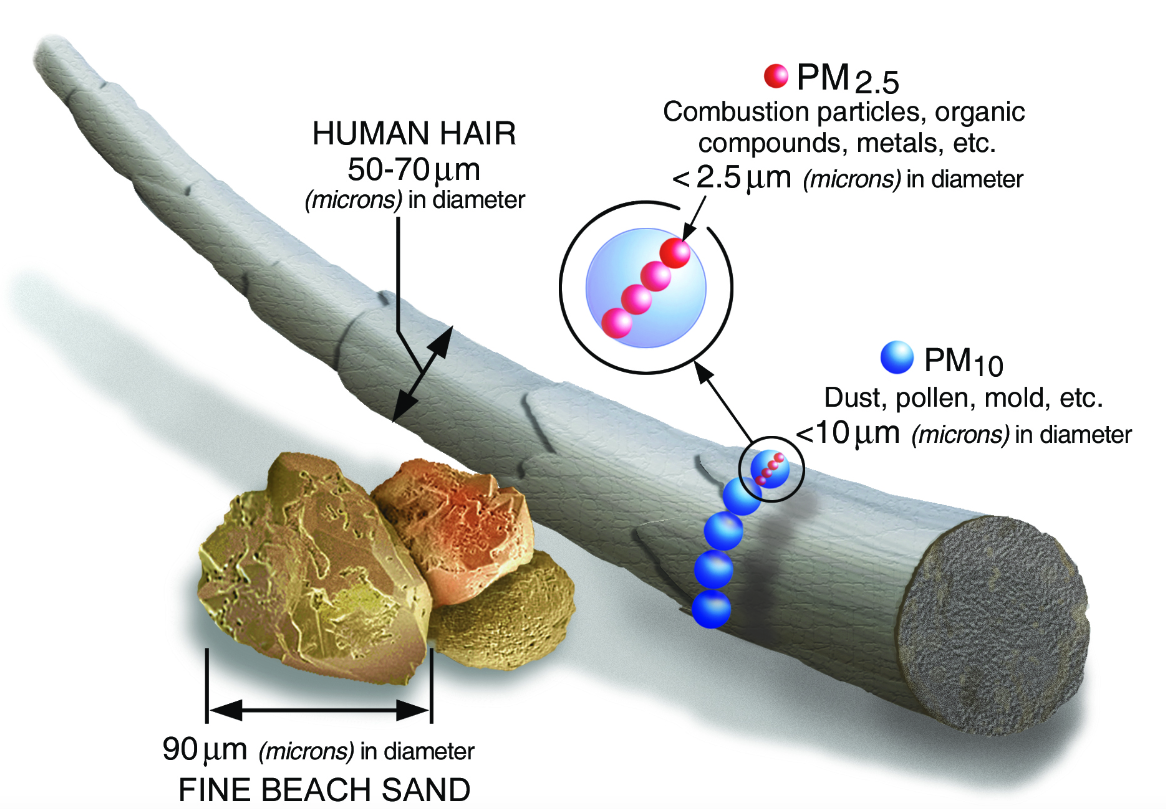
\includegraphics[width=0.75\columnwidth]{introduction/pm-size.png}
  \caption{Size comparisons for PM particles. Image source: US EPA
    (\url{https://www.epa.gov/pm-pollution/particulate-matter-pm-basics}, last
    accessed 2024-09-12).}
  \label{fig:pm-size-scale}
\end{figure}

PM is considered the most important air quality component due to its direct and
widespread impact on public health. Inhaled PM accumulates in the lungs, causing
both short-term and long-term health effects. Fine particulate matter,
specifically PM 2.5, is small enough to pass through the lungs and into the
bloodstream, increasing the risk of cardiovascular diseases, strokes, and cancer
\cite{pm-disease-1, pm-disease-2, pm-cancer}. Due to these combined effects, PM
exposure is estimated to be responsible for millions of premature deaths each
year \cite{pm-mortality-1, pm-mortality-fine}.

In response, many regulatory bodies have introduced new legislation explicitly aimed
at reducing PM levels. The European Union recently revised its air quality
standards to adopt a $10$ $\mu g/m^3$ annual limit for average PM 2.5.
The United States Environmental Protection Agency (EPA) has also adopted tighter
PM regulations, revising its annual PM 2.5 standard to $9$ $\mu g/m^3$ while
maintaining the $35$ $\mu g/m^3$ 24-hour limit.
These developments underscore the growing recognition of the threat posed by PM.


Annual and 24-hour PM regulations are designed to manage long-term exposure but
fail to capture acute spikes from short-term pollution events. These
transient PM spikes can lead to immediate increases in blood pressure, placing
vulnerable populations at heightened risk \cite{pm-bp}. Additionally, short-term
PM exposure has been shown to impair cognitive performance \cite{pm-cognition}.
In fact, the effects of PM on the body are strong enough that short-term PM 2.5
exposure can be independently estimated from a small assortment of biometric
sensors \cite{shawhin-biometrics, shisir-biometrics}. Therefore, high-resolution
PM data are essential for accurately quantifying the immediate impacts of local
PM pollution and facilitating timely mitigation efforts.

\section{Dissertation Goals}

The goal of this dissertation is to advance physical sensing in service of
society by leveraging physically motivated machine learning methods to extract
actionable insights from environmental data. Most modern machine learning models
are designed to solve \textit{general} learning tasks, such as image
classification and language prediction, for which the underly data may come
from a variety of sources with no representation in the real world.
In contrast to these abstract datasets, measurements from physical sensing systems
are governed by physical laws. This requirement imposes a strong constraint on
the space of possible model architectures; the predictions made
for environmental systems must be interpretable in their physical context. We
therefore adopt a physics-based approach, by which we mean machine learning
techniques which strike a balance between data-driven learning and domain-specific
knowledge. This approach includes
\begin{itemize}
\item \textbf{Physically motivated model selection}: The chosen model should
  align with the underlying physical principles of the system under study. For
  example, a model predicting particulate matter should be physically
  realizable so that negative concentrations are disallowed. Similarly, model
  assumptions for the underlying data distribution should apply to the
  measurement data.
\item \textbf{Integration of Prior Physical Knowledge}: Features corresponding
  to relevant physical quantities should be incorporated to improve model
  predictions. For example, the illumination geometry over a water body can
  significantly impact remote sensing imagery, and by extension, the
  estimation of water quality parameters.
\item \textbf{Interpretability}: Understanding \textit{how} a model makes
  predictions is just as important as prediction accuracy. Preference should be
  given to models with explainable structures. Additionally, the quantification of
  model uncertainty is vital for making informed decisions.
\end{itemize}
Towards this end, this work presents a collection of case studies utilizing both
supervised and unsupervised machine learning techniques for the assessment of
water quality and air quality.

In the first category, we are focused on answering the basic question:
\textit{Is this water safe?} Localized in situ measurements for specific water
quality parameters do not provide sufficient spatial coverage to assess water
quality across water bodies with variable topography, composition, and flow. Remote
sensing imagery can cover far wider areas, but simple empirical models
insufficient to robustly map complex spectra to contaminant concentrations. We
therefore utilize machine learning to bridge this gap.

For air quality measurement, our goal is to develop predictive models which can
resolve abrupt pollution spikes in PM time series while \textit{also} enabling
short-term forecasts. Many complicated machine learning models have been
developed for generic time series analysis. In this work, we focus on developing
physically-motivated models based on known PM dynamics. As secondary goal, these
models should be small enough to be deployable on low-cost sensing hardware.


\section{Research Contributions}

The research presented in this dissertation involved the collection of multiple
datasets \textit{and} the creation of software for data processing, modeling,
and analysis. The studies presented in Chapters~\ref{ch:robot-team-supervised}
and \ref{ch:robot-team-gtm} have been published in peer-reviewed journals. The
study from Chapter~\ref{ch:robot-team-gsm} is currently in review, and a
manuscript for the study presented in Chapter~\ref{ch:havok} is in preparation.
A comprehensive list of these various contributions is provided below in
Table~\ref{tab:contributions}


\begin{table}[H]
  \caption{Datasets, software, and publications developed for this dissertation.}
  \label{tab:contributions}
  \begin{center}
    \resizebox{\textwidth}{!}{\begin{tabular}{lccc} \hline
      \textbf{Title} & \textbf{Type} & \textbf{Chapter(s)} & \textbf{Status} \\ \hline
      Autonomous Learning of New Environments with a Robotic Team & & & \\
      Employing Hyper-Spectral Remote Sensing, Comprehensive In-Situ & Article & \ref{ch:robot-team} & published, \cite{robot-team-1}  \\
      Sensing and Machine Learning & & & \\ \hline
      Characterizing Water Composition With an Autonomous Robotic & & & \\
      Team Employing Comprehensive in Situ Sensing, Hyperspectral & Article & \ref{ch:robot-team-supervised} & published, \cite{robot-team-2} \\
      Imaging, Machine Learning, and Conformal Prediction & & & \\ \hline
      Unsupervised Characterization of Water Composition With & & & \\
      Uav-Based Hyperspectral Imaging and Generative Topographic & Article & \ref{ch:robot-team-gtm} & published, \cite{robot-team-gtm} \\
      Mapping & & & \\ \hline
      Generative Simplex Mapping: & & & \\
      Non-linear Endmember Extraction & Article & \ref{ch:robot-team-gsm} & Submitted, In Review \\
      and Spectral Unmixing for Hyperspectral Imagery & & & \\ \hline
      Interpretable Time-delay Embedding Models & & & \\
      for Low-Cost Particulate Matter Sensors: & Article & \ref{ch:havok} & In Preparation \\
      Forecasting and Outlier Detection & & & \\ \hline
      & & & \\
      \texttt{RobotTeam.jl} & Code & \ref{ch:robot-team}, \ref{ch:robot-team-supervised}, \ref{ch:robot-team-gtm}, \ref{ch:robot-team-gsm} & \href{https://github.com/john-waczak/RobotTeam.jl}{Julia Package} \\
      & & & \\ \hline
      & & & \\
      \texttt{SolarGeometry.jl} & Code & \ref{ch:robot-team-supervised} & \href{https://github.com/john-waczak/SolarGeometry.jl}{published, Julia Package} \\
      & & & \\ \hline
      & & & \\
      \texttt{GenerativeTopographicMapping.jl} & Code & \ref{ch:robot-team-gtm}, \ref{ch:robot-team-gsm} & \href{https://github.com/john-waczak/GenerativeTopographicMapping.jl}{published, Julia Package} \\
      & & & \\ \hline
      & & & \\
      \texttt{MLJNonnegativeMatrixFactorization.jl} & Code & \ref{ch:robot-team-gsm} & \href{https://github.com/john-waczak/MLJNonnegativeMatrixFactorization.jl}{published, Julia Package} \\
      & & & \\ \hline
      & & & \\
      HAVOK time series models & Code & \ref{ch:havok} & \href{https://github.com/john-waczak/aq-havok.jl}{Code repository} \\
      & & & \\ \hline

      & & & \\
      Live Air Quality Dashboards & (live) Data & \ref{ch:air-network} & \href{http://mdash.circ.utdallas.edu:3000}{Website} \\
      & & & \\ \hline
      & & & \\
      Air Quality Database & Dataset & \ref{ch:air-network},\ref{ch:havok} & \href{http://mdash.circ.utdallas.edu:8086}{Website} \\
      & & & \\ \hline
      & & & \\
      Robot team Hyperspectral Images & Dataset & \ref{ch:robot-team-supervised}, \ref{ch:robot-team-gtm}, \ref{ch:robot-team-gsm} & \href{https://ncsa.oxn.xsede.org/ees230012-bucket01}{OSN S3 Bucket} \\
      & & & \\ \hline
      & & & \\
      MINTS Air Network Historical Data  & Dataset & \ref{ch:air-network} & \href{https://ncsa.oxn.xsede.org/ees230012-bucket01}{OSN S3 Bucket} \\
      & & & \\ \hline
    \end{tabular}}
  \end{center}
\end{table}



\section{Dissertation Overview}

In Chapter~\ref{ch:robot-team} we first provide a general overview of the
interaction between light and water which motivates the use of hyperspectral imaging
for the assessment of water quality and composition. We then describe a
autonomous robotic team developed to coordinate drone-based hyperspectral imaging
with in situ data collection to greatly accelerate the data acquisition process
for water quality studies. We provide a detailed description of the
georeferencing and reflectance conversion procedures developed to process
hyperspectral images and conclude with an evaluation of total image processing times.

Next, in Chapter~\ref{ch:air-network} we outline measurement techniques for
particulate matter sensing before describing a low-cost network of distributed
air quality monitors designed to collect real-time PM data. We then describe a
containerized data pipeline combining multiple open-source tools to process
network data, provide live visualization dashboards, and enable redundant
data storage.

In Chapter~\ref{ch:robot-team-supervised} we develop a family of supervised
machine learning models to map reflectance spectra to key water composition
parameters. Importantly, this approach utilizes conformal prediction
to assess distribution-free confidence intervals for model predictions. We
examine the relative importance of model features to identify key wavelength
bins for each target variable. Each model is then applied to map the
distributions of physical, chemical, ionic, and biochemical parameters across a
North Texas Pond.

In Chapter~\ref{ch:robot-team-gtm} we expand the capabilities of the robot team
to address situations for which water contaminants are not known in advance. In
this scenario, ground-truth data are not available, and therefore, unsupervised
machine learning methods are needed to identify sources using only hyperspectral
images. We utilize Generative Topographic Mapping for this task and demonstrate
it's ability to visualize the spatial distribution of reflectance spectra across
the water. A rhodamine tracer die released into the pond is then used to
demonstrate that this unsupervised approach successfully identifies unique
spectral signatures which can be used to map contaminant dispersion.

Next, in Chapter~\ref{ch:robot-team-gsm} we present a novel, physics-based
method for unsupervised spectral unmixing and endmember extraction.
This approach builds on the latent variable structure of Generative Topographic
Mapping to directly model linear and nonlinear mixing of radiometric data.
The model is evaluated against Non-negative Matrix Factorization for a
synthetic dataset of mixed spectra from the USGS spectral database. We then
apply the method to unmix water-based hyperspectral images captured by the robot
team. The same rhodamine dye is used to test the ability of the method to map
the dispersion of unknown contaminants across the water.

In Chapter~\ref{ch:havok} we return to the air quality network in order to develop time
series models for local particulate matter data. Given that particulate matter
generally follows a diurnal cycle with intermittent pollution spikes, we
leverage the Hankel Alternative View of Koopman method to simultaneously model
PM time series \textit{and} extract these occasional spikes. We then utilize
this framework to develop short-term forecasting capabilities.

Finally, in Chapter~\ref{ch:future-work} we present directions for future work
before summarizing the conclusions for each study in
Chapter~\ref{ch:conclusions}.




% Big data in the physical sciences
% Comment on the annual data volumes produced by
% \begin{itemize}
%   \item LANDSAT
%   \item Sentinel
%   \item CERN
%   \item James Webb
%   \item SDO AIA
%   \item Medical Imaging (MRI, CT scans, etc...)
% \end{itemize}

% What is machine learning

% Use of machine learning in the physical sciences

% \begin{itemize}
%   \item Remote sensing (inter-instrument calibration, classification, object identification, change monitoring via the NDVI and similar indices, etc.)
%   \item Protein Folding
%   \item Drug discovery
%   \item Surrogate modeling (i.e. for PDE solvers - now very popular at NVIDIA)
% \end{itemize}


% \subsection{Supervised and Unsupervised ML}


% \subsection{Physics-based Machine Learning}




\chapter{Physical Sensing for Environmental Quality Assessment}\label{ch:physical-sensing}

\chapter{Machine Learning Methods}

\chapter{A Coordinated Team of Autonomous Robots for the Rapid Assessment of
  Water Quality}\label{ch:robot-team}

As outlined in Chapter~\ref{ch:intro}, the accurate assessment of water
quality is essential for monitoring ecosystem health and ensuring the safety of
water resources. A plethora of physical parameters
influence local water quality such as turbidity, dissolved organic matter, chlorophyll
concentrations, and suspended particulate matter. Importantly, many of these
contribute measurably to the optical properties of water bodies via
their impact on the scattering and absorption of incident light. Hyperspectral
imaging, which enables the measurement of radiometric quantities
across hundreds of individual wavelength bins, offers a powerful tool for
assessing these parameters. By detecting the subtle variations in
reflectance across the ultraviolet (UV), visible, and Infrared (IR) wavelengths,
hyperspectral imaging enables the differentiation of various water constituents
in complex environments.

In this chapter, we first introduce relevant concepts from radiometry and their
relationship to the measurements made by hyperspectral imagers. We then
describe a variety of physical parameters relevant for the assessment of water
quality and their manifestations in radiometric data. Armed with this
information, we then describe the development of a robotic team incorporating both
drone-based hyperspectral imaging and autonomous in situ data collection with an
autonomous boat. Carefully orchestrating the collection of hyperspectral
images (HSI) coincident with reference data for water quality parameters of
interest allows us to collect data volumes in a few minutes comparable to
decades-long satellite campaigns.

The sensing framework described in this chapter has been published in
\cite{robot-team-1} and was utilized for the studies presented in
Chapters~\ref{ch:robot-team-supervised}, \ref{ch:robot-team-gtm}, and \ref{ch:robot-team-gsm}.


\section{Light and Water}\label{sec:imaging}

Perhaps the greatest achievement of 19th century physics was the unification of
electricity and magnetism by James Clerk Maxwell in which the phenomenon of
light propagation is fundamentally described by oscillations in the electric and
magnetic fields. Therefore, let us first consider a motivating example of
electromagnetic plane waves propagating in a dielectric medium before relating them to
the radiometric measurements made by physical sensors. Recall that Maxwell's
equations in matter are given by
\begin{equation}\label{eq:maxwell}
  \begin{aligned}
    \nabla \cdot \mathbf{D} &= \rho_f, & \nabla \times \mathbf{E} &= - \partial_t \mathbf{B}, \\
    \nabla \cdot \mathbf{B} &= 0, & \nabla \times \mathbf{H} &= \mathbf{J}_f + \partial_t\mathbf{D},
  \end{aligned}
\end{equation}
where $\rho_f$ is the free charge density and $\mathbf{J}_f$ is the free current
density. For linear media of permittivity $\epsilon$, and permeability $\mu$, we
have $\mathbf{D}=\epsilon\mathbf{E}$ and $\mathbf{H}=\frac{1}{\mu}\mathbf{B}$.
In a region where $\rho_f=0$ and $\mathbf{J}_f=0$, these equations reduce to the
wave equation for $\mathbf{E}$ and $\mathbf{B}$, admitting traveling plane-wave
solutions.

A monochromatic plane-wave traveling in the $\hat{x}$ direction is given by
\begin{equation}\label{eq:travelling-wave}
  \begin{aligned}
    \mathbf{E} &= \bar{E}_0\exp(i(\kappa x - \omega t))\hat{y}, \\
    \mathbf{B} &= \bar{B}_0\exp(i(\kappa x - \omega t))\hat{z},
  \end{aligned}
\end{equation}
where $\bar{E}_0$ and $\bar{B}_0$ are complex numbers
(absorbing the phase). Equation~\ref{eq:travelling-wave} trivially satisfies
$\nabla \cdot \mathbf{D} = 0$ and $\nabla \cdot \mathbf{B} = 0$. Substitution into
the remaining equations yields the familiar dispersion relation for
electromagnetic waves:
\begin{equation}
  \kappa^2 = \omega^2\mu\epsilon
\end{equation}

Allowing for $\sqrt{\mu\epsilon}$ to be complex, we can decompose $\kappa$ into
\begin{equation}
  \kappa = \frac{2\pi m}{\lambda}
\end{equation}
where $m=n - ik$ is the \textit{complex index of refraction}. Substituting this expression
into Equation~\ref{eq:travelling-wave} and taking the real part, we obtain
\begin{equation}\label{eq:wave-real}
  \begin{aligned}
    \mathbf{E} &= E_0\exp\left(-\frac{2\pi k x}{\lambda}\right)\cos\left(  \frac{2\pi n x}{\lambda} - \omega t  + \phi \right) \hat{y} \\
    \mathbf{B} &= B_0\exp\left(-\frac{2\pi k x}{\lambda}\right)\cos\left(  \frac{2\pi n x}{\lambda} - \omega t  + \phi \right) \hat{z} \\
  \end{aligned}
\end{equation}

Instruments like the hyperspectral imagers do not measure
the time-dependent amplitudes of the electric and magnetic fields. Instead, they
detect energy deposited through a surface carried by these fields. This energy
flow is characterized by the Poynting vector, $\mathbf{S} =
\frac{1}{\mu}\mathbf{E}\times\mathbf{B}$ which has units of $W/m^2$, in other
words, the energy flux through a surface. Additionally, the sample rates of realistic
instruments are much longer than oscillations in $\mathbf{E}$ and $\mathbf{B}$ so
that the time-averaged Poynting vector $\langle
\mathbf{S} \rangle$ is really measured. Given that $\langle  \cos^2(\theta) \rangle =
1/2$, this results in
\begin{equation}
  \langle \mathbf{S} \rangle = \frac{1}{2}\sqrt{\frac{\epsilon}{\mu}}E_0^2\exp\left(-\frac{4\pi k x}{\lambda}\right) \hat{x}
\end{equation}

Here we see an important consequence of considering a complex index of reaction:
the quantity $a(\lambda)=4\pi k/\lambda$ is called the \textit{absorption coefficient}
which characterizes the amount of incident radiation absorbed by the medium as a
function of the penetration distance $x$. In low-turbidity coral reefs this helps
explains why red colors become muted at increasing depths. Finally, we note that
for a homogeneous solution containing $n$ chemicals, the Bouguer-Beer-Lambert law
relates the total absorption coefficient to each chemical concentration via
\begin{equation}
  a(\lambda) = \sum_i^n c_i\varepsilon_i(\lambda)
\end{equation}
where $c_i$ is the concentration of the $i$-th chemical species in the solution,
and $\varepsilon_i(\lambda)$ is the wavelength-dependent molar absorption
coefficient. The connection between the concentration of constituents in the
water to the interaction of a mixture with incident light motivates the
assessment of water quality by spectroscopic techniques.

\subsection{Radiometry}

\textit{Radiometry} is the science of the measurement of electromagnetic energy
and involves a number of derived quantities. As outlined in the previous
section, most optical and spectroscopic instruments do not directly measure the
oscillations in the electric and magnetic fields, but rather the energy they
transport into a sensing element. 

The \textit{spectral radiance} is defined as
\begin{equation}
  L(\mathbf{x}, t, \hat{\xi}, \lambda) = \frac{\partial^4 Q}{\partial t \partial A \partial \Omega \partial \lambda},
\end{equation}
or in words, the amount of incident radiant energy per area per
second, per solid angle, per wavelength. Importantly, the spectral radiance
depends on the sampling position $\mathbf{x}$ and time $t$ as well as the wavelength
$\lambda$ and direction of light $\hat{\xi}$. Historically many different
conventions for naming radiometric quantities have been used. We follow the
conventions used in \cite{mobley-text} for which the prefix \textit{spectral} is
used to indicate the explicit \textit{per-wavelength} dependence of a
radiometric quantity. $L$ is the fundamental measured quantity which captures
the spatial, temporal, spectral, and orientation dependencies of the light field.

When an instrument samples light from \textit{all} possible directions passing
through a collection area, then the
measured quantity is the \textit{spectral radiance}. Naturally, this quantitiy
depends on the orientation of the sensor. For example, the \textit{downwelling
  spectral radiance}, $E_d$ is defined by
\begin{equation}
  E_d(\mathbf{x}, t, \lambda) = \int_0^{2\pi} \int_0^{\pi/2}L(\mathbf{x}, t, \theta, \phi, \lambda)\cos\theta \sin\theta d\theta d\phi
\end{equation}
where the factor of $\cos\theta$ accounts for the apparent area at an angle
$\theta$ from the surface normal.

Different materials lead to different distributions of scattered light. For
\textit{specular} materials such as polished mirrors or the air-water interface, light
reflected at the surface leaves at an angle identical to the angle of incidence.
The polar opposite of a specular material is a \textit{Lambertian}, or perfectly
diffuse material. Light scattering off of a Lambertian surface is distributed
equally in all directions so that $L$ is independent of $\theta$ and $\phi$. As
a consequence, the spectral irradiance of light from a Lambertian surface is
\begin{equation}
  E = \int_0^{2\pi}\int_0^{\pi/2} L(\mathbf{x}, \lambda)\cos\theta \sin\theta d\theta d\phi = \pi L
\end{equation}

Given measurements for the downwelling (incident) and upwelling spectral
irradiances, the \textit{reflectance} is defined by their ratio:
\begin{equation}
  \rho(\mathbf{x},\lambda) = \dfrac{E_u(\mathbf{x}\lambda)}{E_d(\mathbf{x}, \lambda)}.
\end{equation}
This quantity is valuable as it extracts the useful signal from an image by
\textit{dividing out} the spectrum from the lighting source, in this case,
incident solar radiation.

\subsection{Optical Properties of Water Bodies}\label{sec:optical-properties-water}

The formulation of Maxwell's equations in Equation~\ref{eq:maxwell} treats
macroscopic media as continuous. However, at atomic scales, bodies of water
consist of collections of molecules (\ce{H2O} and other dissolved substances)
together with particulates which vary in size. The interaction of light with
these particles can be approximated by the interaction of light with dielectric
spheres with a specific radius and (potentially complex) index of refraction.
The general solution for the scattered intensity field of light by a dielectric
sphere of \textit{any} radius is known as \textit{Mie Theory} and involves
highly complicated expressions of infinite series of spherical multi-pole
expansions which can be evaluated numerically.

A special case for elastic scattering by particles with a diameter $d <<
\lambda$ is known as \textit{Rayleigh Scattering}. In this regime, the scattered
intensity obeys
\begin{equation}
  I = I_0  \left( \frac{2\pi}{\lambda} \right)^4 \left( \frac{d}{2} \right)^6 \left( \frac{1 + \cos^2\theta}{2R^2} \right)
\end{equation}
where $\theta$ is the scattering angle, $R$ is the distance from the particle to
the measurement point, and $n$ is the (real) index of refraction. Lord Rayleigh
used the $\lambda^{-4}$ dependence of this expression to explain why the sky is
blue: atmospheric particles (which we now understand to be gas molecules) with
diameters much smaller than visible wavelengths scatter blue light
much more than red light.

In addition to scattering, molecules and particulates can absorb incident light
according to their specific structure. For pure water, electronic transitions
lead to absorption in the UV while rotational and vibrational modes are relevant
at longer wavelengths. Critically, there is a transparent \textit{window} of low
absorption for visible wavelengths which enables aquatic life to access solar
energy.

Water bodies contain a variety of constituents leading to a continuous size
distribution from chemicals at the atomic scale ($\sim$$0.1$ nm) to virus
($\sim$$100$ nm), to aquatic animals ($\sim$$1$ m). These components are traditionally
classified into dissolved or particulate matter of organic or inorganic origin.
Most water bodies contain a variety of dissolved salts. For ocean waters these
account for roughly 3.5\% by weight while fresh water bodies tend to contain
trace amounts. Natural waters also contain a variety of dissolved organic
compounds produced by the decay of plant matter. These compounds mostly include
fulvic and humic acids which impart a yellowish-brown color in sufficient
conecntrations and are referred to in the literature as \textit{colored
  dissolved organic matter} (CDOM) \cite{cdom-acids}. Inorganic particulate
matter in natural waters is largely due to the weathering of rocks in soils
while organic particulates include bacteria, phytoplankton, zooplankton, and
larger organic detritus.

Light absorption by CDOM can be reasonably modeld using an exonential function
of the form
\begin{equation}
  a(\lambda) = a(\lambda_0)\exp(-S_g(\lambda - \lambda_0))
\end{equation}
for a reference wavelength $\lambda_0$ \cite{aurin2018remote}. The exact
value of the spectral slope $S_g$ depends on the proprotions of specific types
of CDOM with typical values on the order of $\sim$$0.01$.

Absorption by phytoplankton and many other organic sources is largely due to
photosynthetic pigments with cells such as chlorophyll. Chlorophyll a
absorption is strongest for blue and red wavelengths with peaks at
$\lambda\approx 430$ nm and $\lambda\approx 665$ nm, respectively. Other
relevant pigments include phycoerythrin and phycocyanin  which occur in
blue-green algae. Estimations of their concentration from remote sensing imagery
has been used to track the evolution of harmful algal blooms which often occur
due to increased nutrient concentrations from agricultural and urban runoff
\cite{algal-blooms-rs}.

Lastly, we note that in addition to scattering and absorption, many chemicals
such as crude oil and organic components such as CDOM and chlorophyll undergo
fluorescence when excited at appropriate wavelengths. For example, CDOM excited
by UV light with $\lambda\in[250, 400]$ nm will emit at wavelengths in
$\lambda\in[400, 500]$ depending on the specific types of organic compounds
\cite{cdom-fluorescence}. Fluorometers calibrated for these excitation
and emission properties can therefore be used for in situ assessment of many
water constituent concentrations.

\section{Coordinated Robot Teams}

For decades, multi-spectral imagers which sample a small number of
broad wavelength bands have seen widespread use in
the remote sensing community as a means to take advantage of the wealth of
information contained in the reflectance spectra of materials. Multi-spectral imagers,
like those deployed on MODIS, Sentinel 2, and other satellite platforms, include
wavelength bands ranging from the near-UV,
through the visible spectrum, and into the Infrared and have been applied in a
variety of domains from tracking land change, characterizing deforestation,
monitoring erosion, evaluating crop health, and many others
\cite{remote-sensing-foliage, remote-sensing-applications, thenkabail-indices}.

\begin{figure}[!hbt]
  \centering
  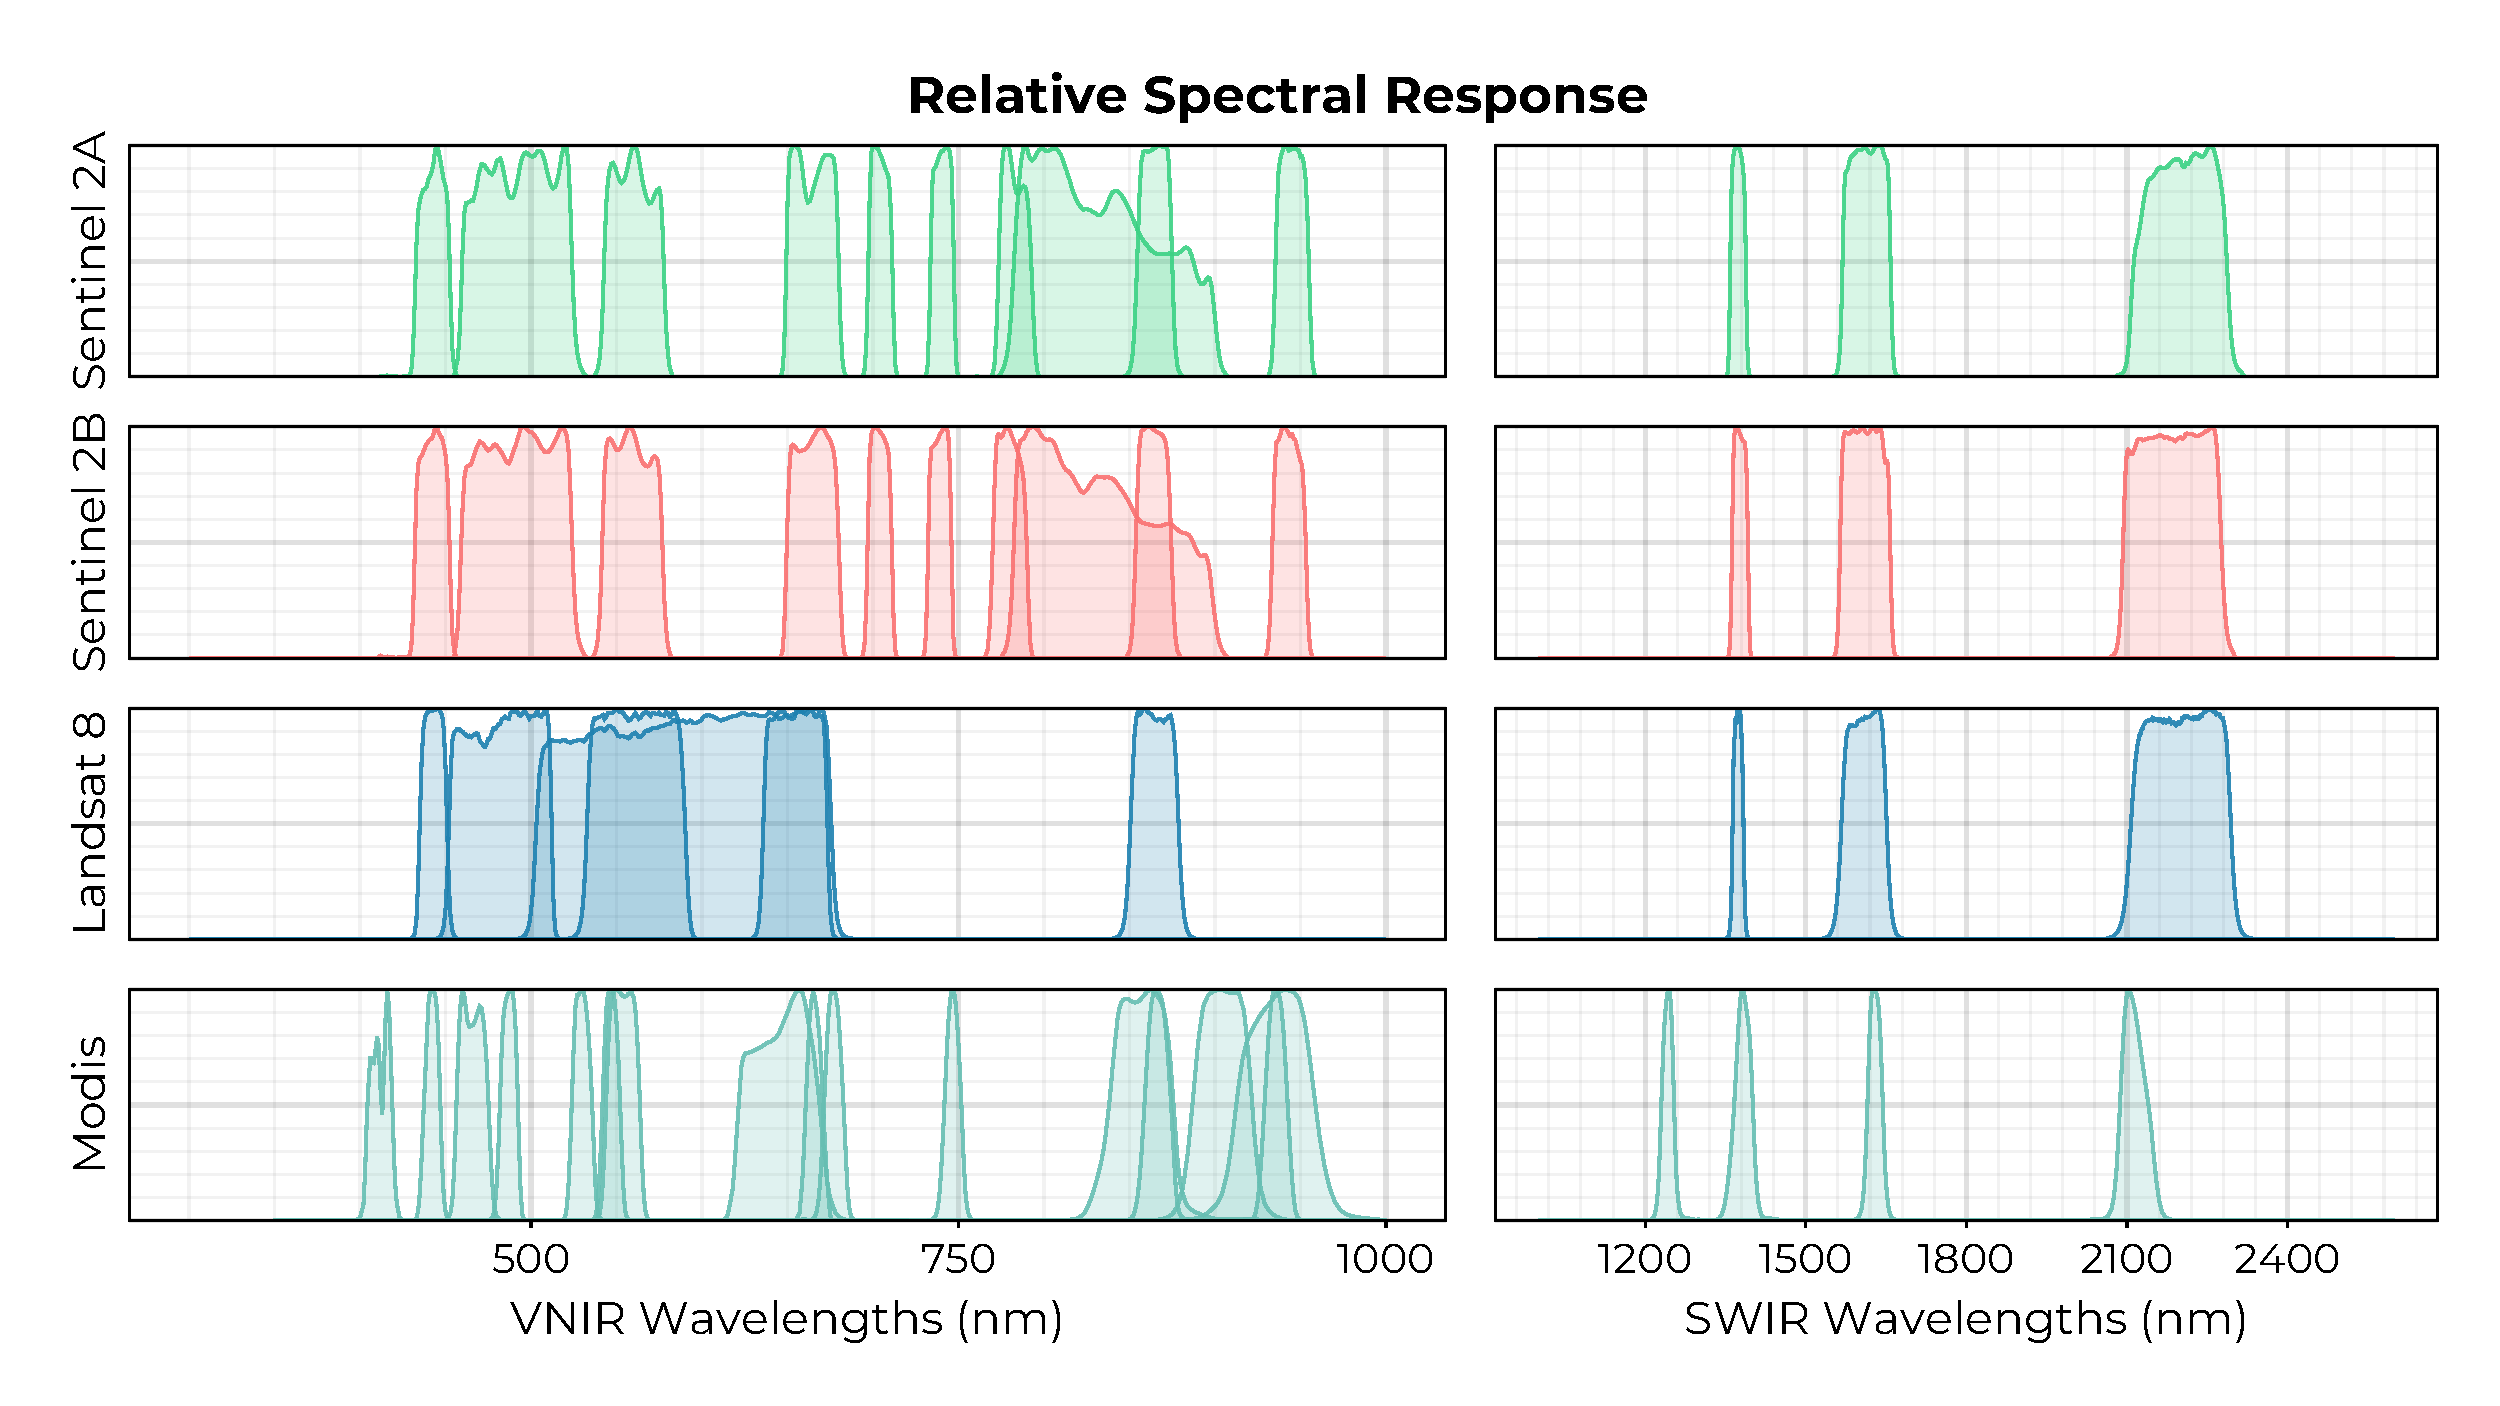
\includegraphics[width=0.85\columnwidth]{robot-team/passbands.pdf}
  \caption{A comparison of the relative spectral response for the passbands of popular multi-spectral imaging remote sensing platforms.}
  \label{fig:passbands}
\end{figure}

Many currently used spectral indices like the normalized difference vegetation
index (NDVI) take advantage of spectral features by comparing ratios of
pigment sensitive passbands to the stable signals in the infrared to infer the
abundance of chlorophyll, and consequently, the health of plants
\cite{ndvi-chlorophyll}.  However, despite the many successful
applications of multi-spectral imaging, there are a few key limitations which
impact their use for the assessment of water quality.

\begin{enumerate}
  \item Multi-spectral imagers have limited use for the assessment of many
    constituents affecting water quality whose spectral features overlap in the
    broad wavelength bands of systems like those shown in Figure~\ref{fig:passbands}.
  \item Satellite-based instruments measure top of atmosphere reflectance and
    must be carefully corrected to obtain values at the surface by accounting for
    absorption and scattering by atmospheric gases and particulates.
  \item Validating models which map remotely sensed reflectance to parameters of
    interest requires the collection of in situ reference data. This relies on
    serendipetous satellite passes over sensing sites often requiring decades of
    observations to collect sufficient quantities needed for model training and
    validation \cite{aurin2018remote, ross2019aquasat}.
\end{enumerate}

Hyperspectral imagers are designed to measure spectral radiance for many
hundreds of wavelengths at each image pixel. Their improved spectral resolution
makes it possible to detect fine spectral features. Developments in
hyperspectral imaging technology have led to dramatic reductions in both their
size and weight so that it is now possible to incorporate the
technology as the payload of highly mobile unmanned aerial vehicles (UAV) such as
drones. By collecting hyperspectral images (HSI) close to the ground, we limit
the need for complicated atmospheric corrections while enabling centimeter-scale
spatial resolutions. However, the massive size of HSI poses a significant
computational challenges for their adoption in real-time
applications.

The typical timescale from starting work on a new remote sensing data
product to its operational readiness is at least a couple of years, but, more
typically, a decade or more. Our goal is to reduce this timescale to be near
real time by utilizing an autonomous robotic team that can both collect the
training data, and then in real time process and stream the remote sensing data
products. The fully autonomous team includes an uncrewed surface vessel (USV)
that carries a suite of sensors to measure in situ water composition,
and an autonomous UAV equipped with a hyperspectral imager, downwelling
irradiance spectrometer, thermal imagers, and embedded compute for onboard machine
learning capabilities. Figure \ref{fig:drone-team} shows photographs of the robot team
during a deployment in North Texas.

\begin{figure}[!hbt]
  \centering
  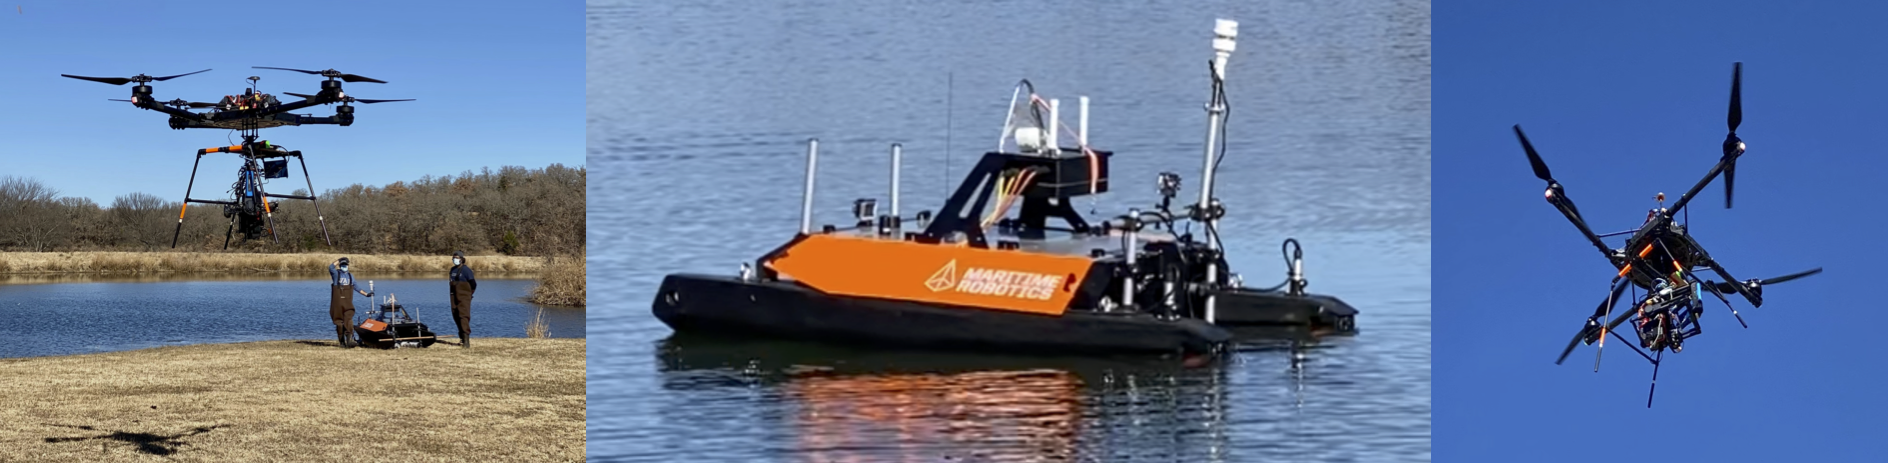
\includegraphics[width=0.9\columnwidth]{robot-team/robot-team-photos.png}
  \caption{The autonomous robotic team. (\textbf{left}) The drone hovering a few
  feet above the ground during take-off. (\textbf{center}) the USV deployed in
  the water. (\textbf{right}) The drone as seen from below.}
  \label{fig:drone-team}
\end{figure}

The autonomous boat used is a
\href{https://www.maritimerobotics.com/otter}{Maritime Robotics Otter }. With a
footprint of only 200 × 108 × 81.5 cm, a weight of 55 kg, and dual electrical
fixed thrusters, it is an easily deployable asset that can be transported in a
van or even within normal airliners to a survey site. At a cruise speed of two
knots, it has a duration of approximately 20 hours per battery charge. It can use
WiFi, cellular, and an optional AIS receiver for communication to the control
station. Our drone is a \href{https://freeflysystems.com/alta-x}{Freefly Alta-X}
professional quad-copter. It was specifically designed to carry cameras, with a
payload capacity of up to 35 lb, a long range data link, and autonomy provided
by the Open PX4 flight stack. The open source QGroundControl software is used to
control the autonomous operations.

Both the UAV and USV carry high-accuracy GPS and inertial
measurement units (IMU) so that every data point can be georeferenced and time
stamped. Each robot can also join the same wireless network which connects the
robots and a ground control stations. For the deployments described in
Chatpers~\ref{ch:robot-team-supervised}, \ref{ch:robot-team-gtm}, and
\ref{ch:robot-team-gsm}, long-range
\href{https://www.ui.com}{Ubiquiti 5 GHz LiteBeam airMAX WiFi} was used for
data transfer and control. The network
also includes a local \href{https://www.synology.com}{Synology network-attached
  storage (NAS)} device which syncs collected data to another NAS in our home laboratory at the
UT Dallas for redundancy.

The robotic boat payload includes a
\href{https://www.biosonicsinc.com/products/mx-aquatic-habitat-echosounder/}{BioSonics
  MX Aquatic Habitat Echosounder sonar} for rapid assessment and mapping of
aquatic vegetation, substrate and bathymetry. Three
\href{https://www.waterprobes.com/multiprobes-and-sondes-for-monitori}{Eureka
  Manta-40 multi-probes}, a
\href{https://www.sequoiasci.com/product/lisst-abs/}{Sequoia Scientific
  LISST-ABS acoustic backscatter sediment sensor}, and an
\href{https://www.airmar.com/weather-description.html?id=153}{Airmar Technology
  Corporation 220 WX ultra-sonic weather monitoring sensor}.

The first Manta-40 multi-probe includes sensors for temperature and turbidity
and
\href{https://www.turnerdesigns.com/cyclops-7f-submersible-fluorometer}{Turner
  Designs Cyclops-7 submersible Titanium body fluorometers} for chlorophyll a,
chlorophyll a with red excitation, blue-green Algae for fresh water
(phycocyanin), blue-green Algae for salt water (phycoerythrin), and CDOM.
The second Manta-40 multi-probe includes sensors for temperature, conductivity
(with specific conductance, salinity, and total dissolved solids, TDS), pH (with
separate ref-erence electrode), optical dissolved-oxygen, turbidity, and ion
selective electrodes by Analytical Sensors and Instruments
(\url{http://www.asi-sensors.com/}, accessed 05/01/2021) for ammonium
(\ce{NH4^+}), bromide (\ce{Br^-}), calcium (\ce{Ca^2+}), chloride (\ce{Cl^-}),
nitrate (\ce{NO3^-}), and sodium (\ce{Na^+}). The third Manta-40 multi-probe
includes sensors for temperature, turbidity, a total dissolved gas sensor, and
additional fluorometers for measuring optical brighteners, crude oil, refined
fuels, and tryptophan.

\begin{figure}[!hbt]
  \centering
  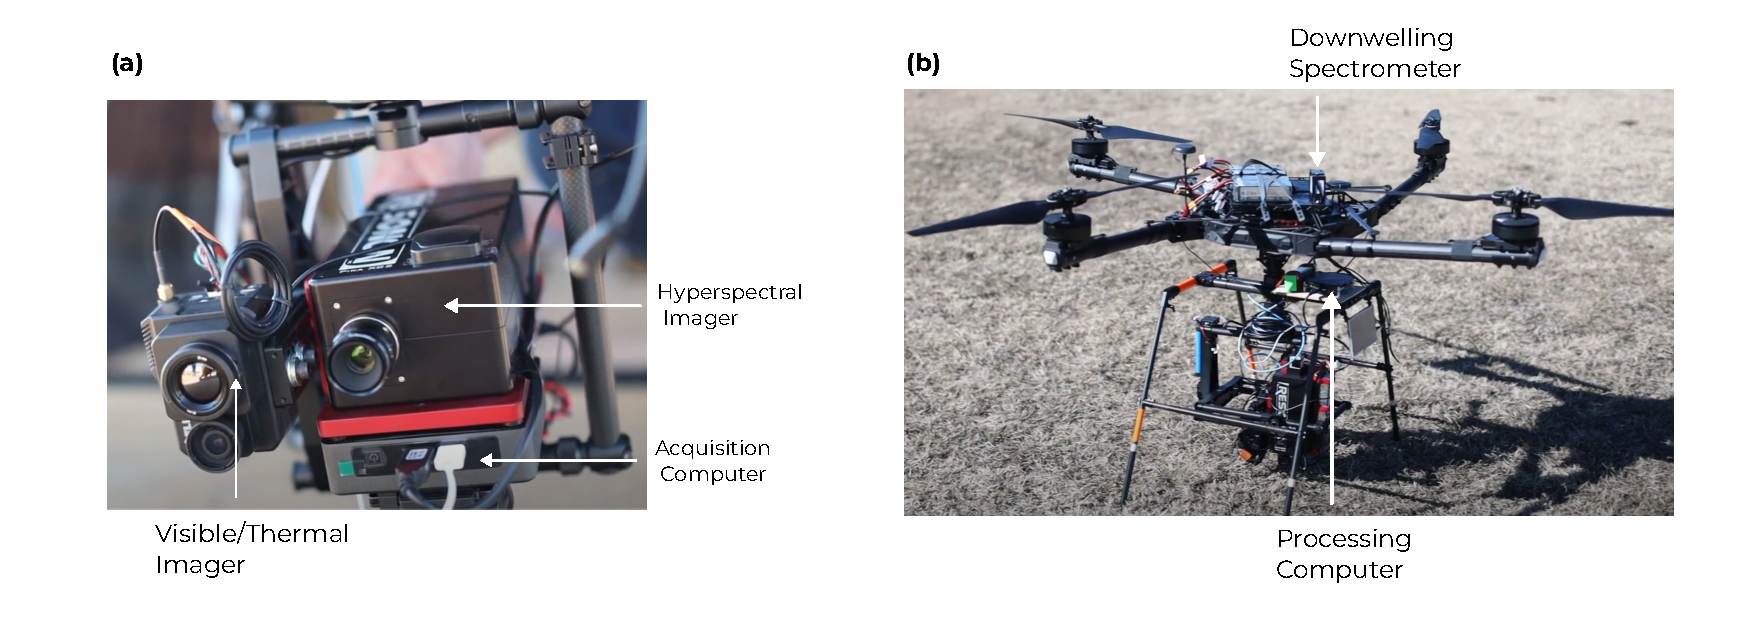
\includegraphics[width=0.9\columnwidth]{robot-team/annotated-drone.pdf}
  \caption{An annotated view of the autonomous drone showcasing the hyperspectral imager and onboard compute.}
  \label{fig:uav-closeup}
\end{figure}

Custom landing gear gear made from light-weight
carbon fiber was manufactured for the UAV to maximize the potential carry
capacity. The installed hyperspectral imager is a
\href{https://resonon.com/Pika-XC2}{Resonon Visible+Near-Infrared (VNIR) Pika
  XC2}, and thermal images are captured with
a \href{https://www.flir.com/products/duo-pro-r/}{FLIR Duo Pro R} installed
in a parallel configuration as indicated in Figure~\ref{fig:uav-closeup}. On top
of the UAV, a sky facing Ocean Optics UV-Vis-NIR spectrometer with an included
cosine corrector measures the incident downwelling irradiance to enable the
conversion of radiance hyperspectral data cubes to reflectance.

During a single 30 minute deployment, the robot team is able to autonomously
collect over a terabyte of HSIs together with over 10,000 in situ measurements
from the suite of sensors on the USV. Coordinating UAV flights to overlap USV
data collection makes it easy to identify reflectance spectra collocated with
USV measurements. This in turn makes it possible quickly train machine learning
models mapping HSI reflectance spectra to water quality parameters of interest.
Once trained, the models may be deployed directly onto the UAV computer to allow
streaming of concentration maps to the ground station during subsequent flights.
The machine learning models developed for the robot team are described in
Chapter~\ref{ch:robot-team-supervised}. Additionally, unsupervised techniques
for assessing the presence of unanticipated contaminants are developed in
Chapters~\ref{ch:robot-team-gtm} and
\ref{ch:robot-team-gsm}.

In the final sections of this chapter, we present the methods implemented to
rapidly georectify captured HSI and convert their radiance measurements to
reflectance using secondary spectra from the downwelling irradiance
spectrometer. This process quickly assigns latitude and longitude coordinates to
each HSI pixel making it possible to generate maps of the reflectance
distribution across an entire body of water. The coordiantes of georectified HSI
are also used to collocate reflectance spectra with in situ USV measurements.



\section{Rapid Processing and Georectification of Hyperspectral Data Cubes}

For an HSI platform to operate in (near) real-time, three key tasks are critical:
\begin{enumerate}
\item \textbf{FileIO}: Raw HSI need to be quickly read by the on-board processing computer.
\item \textbf{Georectification}: HSI must be georeferenced so that each image
  pixel can assigned a location on the ground.
\item \textbf{Radiometric Conversion}: HSI data cubes need to converted to the
  desired radiometric quantity, i.e. the reflectance.
\end{enumerate}

The first item is readily accomplished by means of light-weight, high-volume
solid state drives incorporated into the UAV computer. To address the second, we
need both sufficient compute capabilities and optimized processing software. The
final item relies on both the georectified data cube and the secondary
irradiance spectrum captured by the upward facing downwelling irradiance
spectrometer. To enable this workflow, the UAV utilizes a pair of light-weight
processing computers (Intel NUCs) each have 12 cores and 64 gigabytes of
installed RAM.  One is attached directly to the imager and
manages data acquisition by the camera and saving of raw HSI files. The second
NUC is mounted above the payload and serves as the onboard data processing unit. These
computers can be seen in panels (a) and (b) of Figure~\ref{fig:uav-closeup}.

%The upward facing spectrometer captures the \textit{downwelling} irradiance
%spectrum, $E_d(\lambda)$ which is necessary to enable conversion from radiance units to the

The georectification procedure implements for HSI from the UAV is based on the
methods described in \cite{muller2002program, baumker2001new, mostafa2000multi}
for pushbroom-mode hyperspectral imagers while the reflectance conversion
assumes Lambertian scattering as described previously in Section~\ref{sec:imaging}.
The processing steps are as follows:

\begin{enumerate}
\item Raw imagery (radiance spectra) are continuously captured by the hyperspectral imager and stored in binary ENVI format.
\item The processing computer read an ENVI file into a multi-dimensional array
  once it finishes writing.
\item Associated flight data (GPS and IMU) are read.
\item Flight data are interpolated to match the sample times for each HSI scan-line.
\item Each scan-line is georeferenced to obtain coordinates (lat,lon) for each pixel.
\item The georeferenced HSI is then resampled to a regular grid spatial grid.
\item The downwelling irradiance spectrum associated with the HSI is read.
\item The downwelling spectrum is interpolated to match the wavelength bins of the HSI
\item The HSI is converted o reflectance.
\item Spectral indices (NDVI, etc...) are computed.
\item The final data cube is saved to an HDF5 file.
\end{enumerate}
A visual representation of the pipeline is shown in
Figure~\ref{fig:hsi-pipeline} below.
\begin{figure}[H]
  \centering
  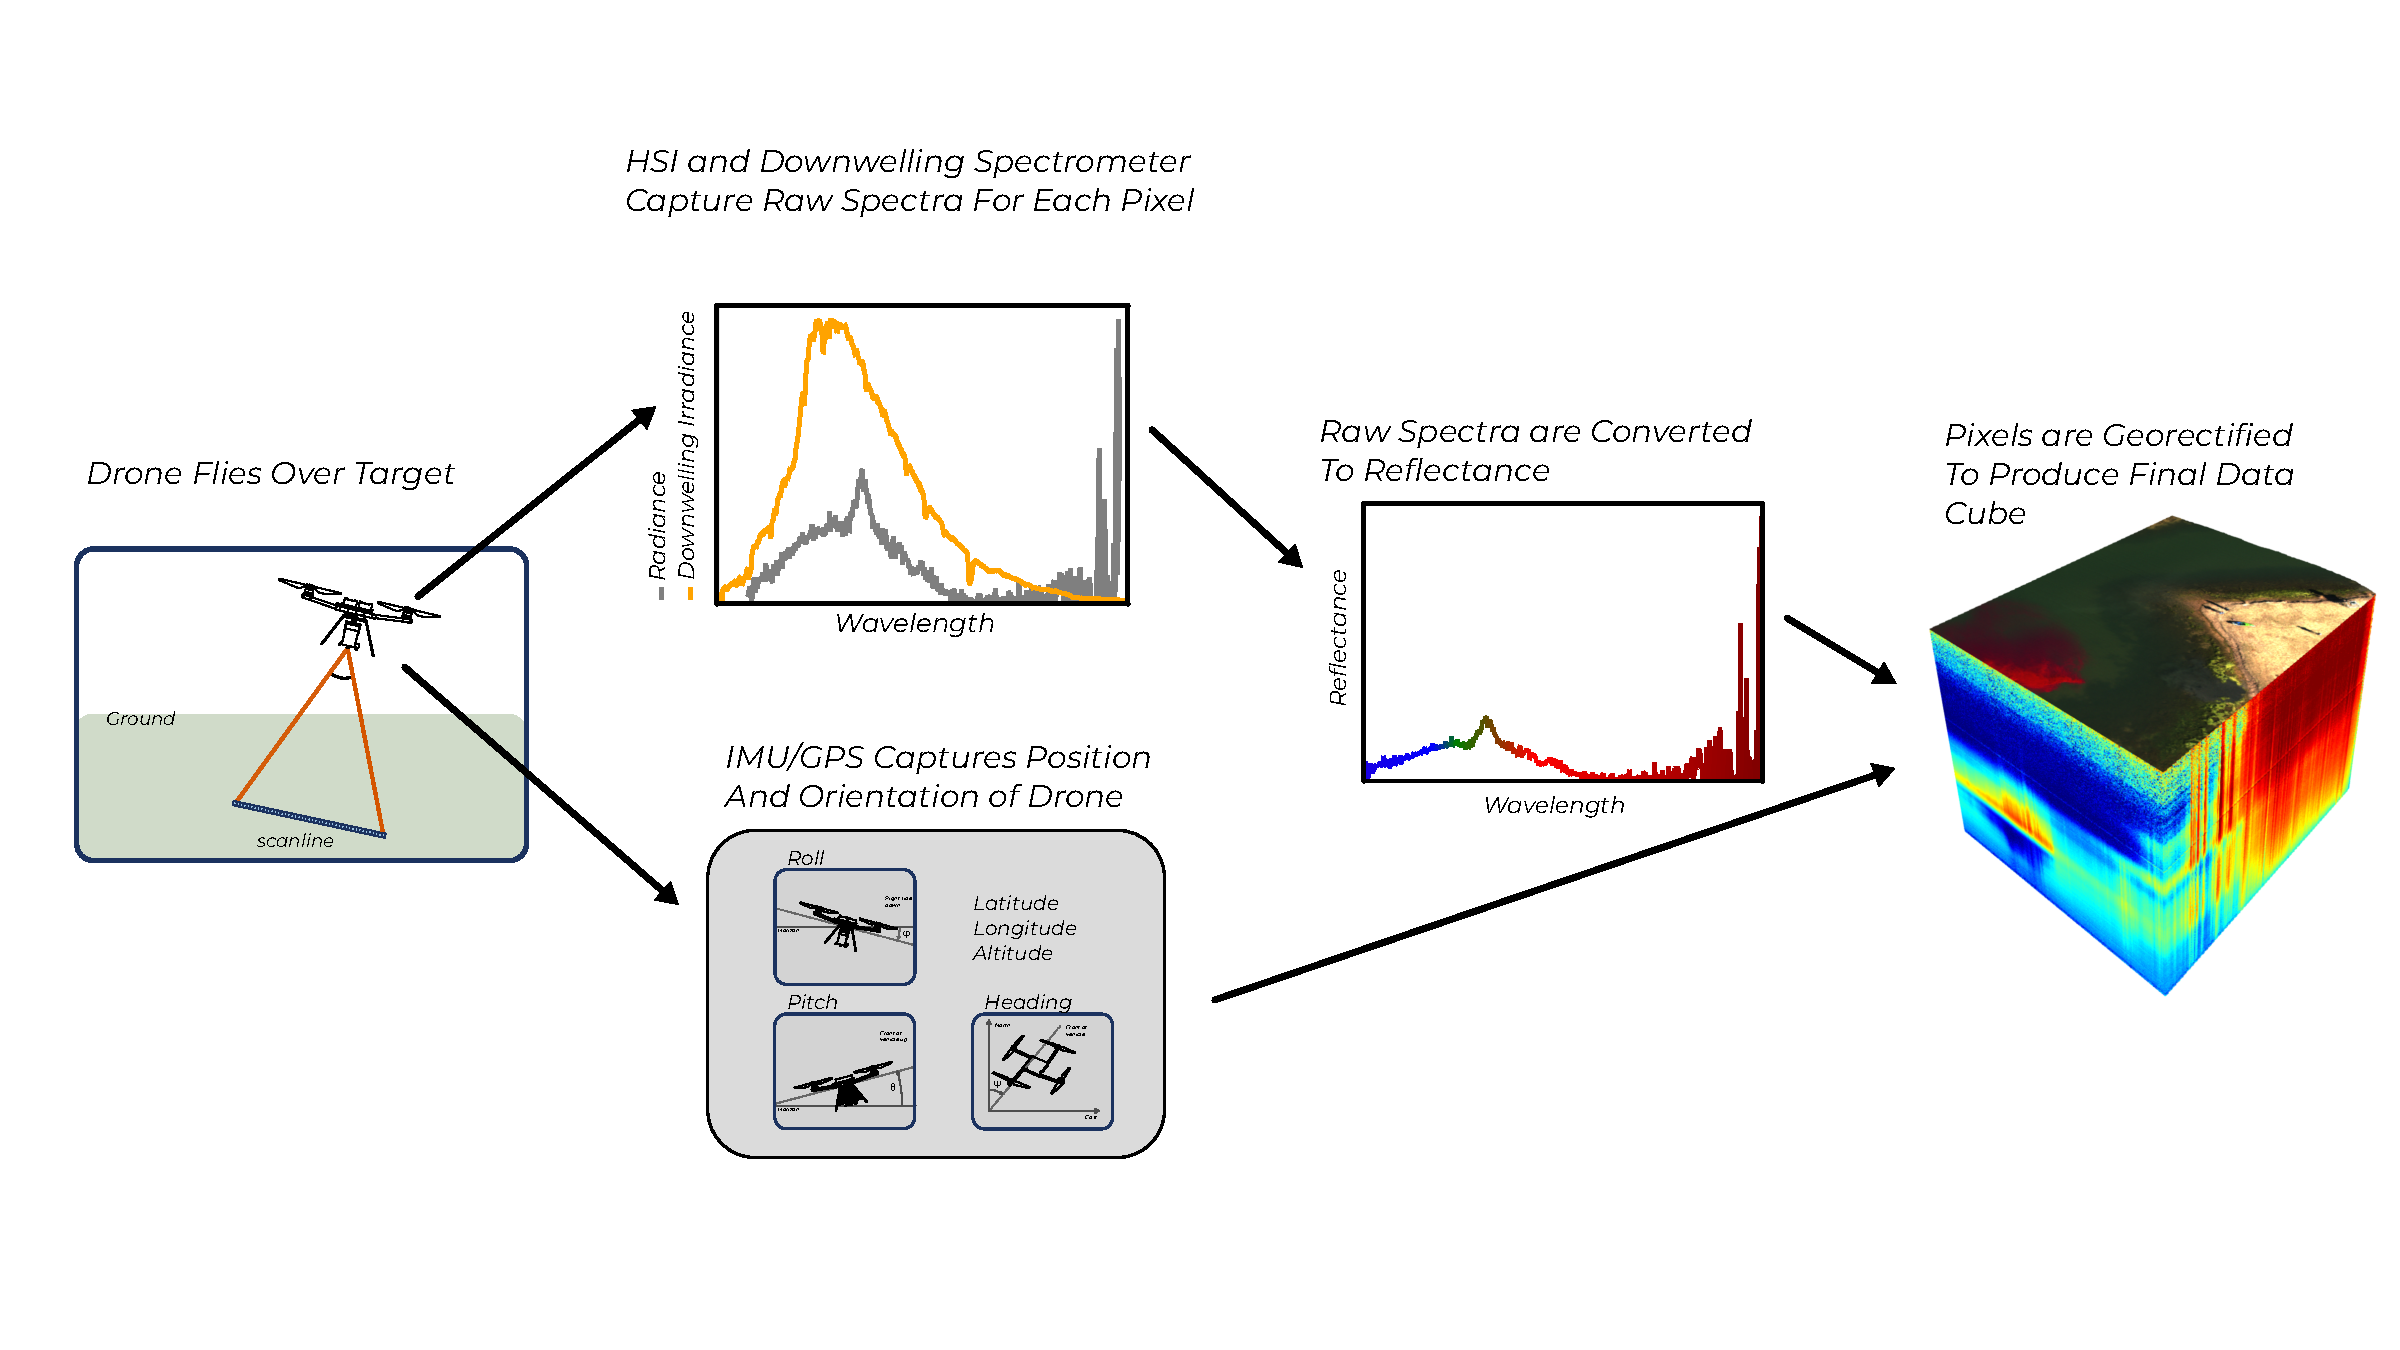
\includegraphics[width=\columnwidth]{robot-team-supervised/materials-and-methods/pipeline-figure-2.pdf}
  \caption{Hyperspectral image processing: Hyperspectral data cubes are
    collected one scan-line at a time (left). By utilizing downwelling
    irradiance spectra, we convert each pixel from spectral radiance to
    reflectance. By using orientation and position data from the on-board GPS
    and INS, we georeference each pixel to assign it a latitude and longitude on
    the ground. The final data product is the georectified hyperspectral
    reflectance data cube (right) visualized as a pseudo-color image with
    reflectance  as a function of wavelength along the
    z-axis.\label{fig:hsi-pipeline}}
\end{figure}


% \begin{figure}[h]
%   \centering
%   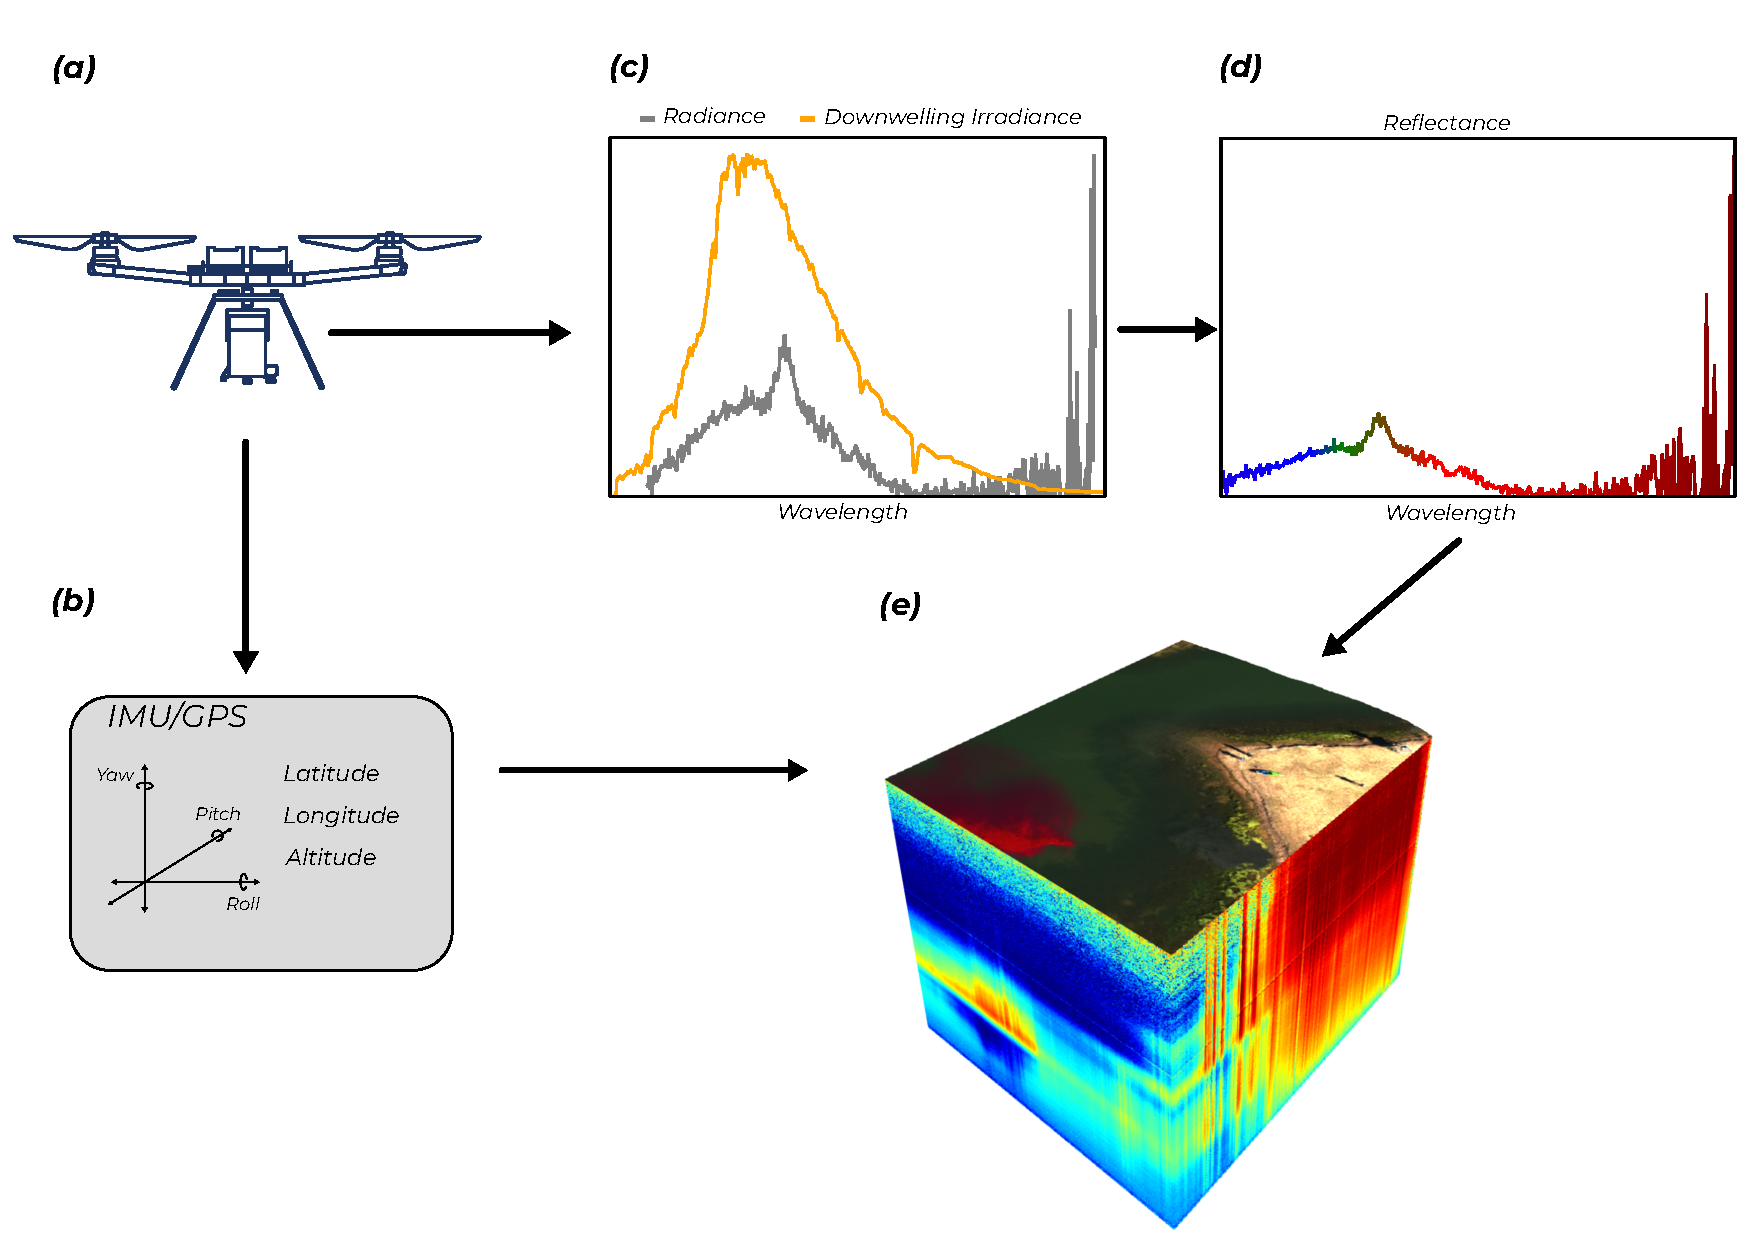
\includegraphics[width=0.85\columnwidth]{robot-team/georectification/pipeline-figure.pdf}
%   \caption{Visual representation of the HSI processing pipeline. HSI images from
%   the UAV (a) are georectified using position and orientation data from the
%   embedded GPS/IMU unit (b). Pixel radiance spectra are combined with
%   downwelling irradiance (c) to yield a reflectance spectrum for each pixel (d).
%   The result is a georectified reflectance data cube (e).}
%   \label{fig:hsi-pipeline}
% \end{figure}


\subsection{Georeferencing and Resampling}

The hyperspectral imager used on the UAV is different from a typical camera;
instead of capturing an image by sampling light across array of sensors, the
hyperspectral imager uses a pushbroom configuration. In this setup, a single
scan-line of pixels is captured by the sensor for each wavelength and an image
is formed as the drone flies along its route. This poses an interesting
challenge for georeferencing as each individual scanline must be transformed
independently. As the drone's path winds and turns, each scanline
is stretched and rotated based on the relative orientation of
the drone to the ground at the time of capture. This sampling geometry as well
as the relevant orientation angles are illustrated in Figure
\ref{fig:georectification}.

\begin{figure}[h]
  \centering
  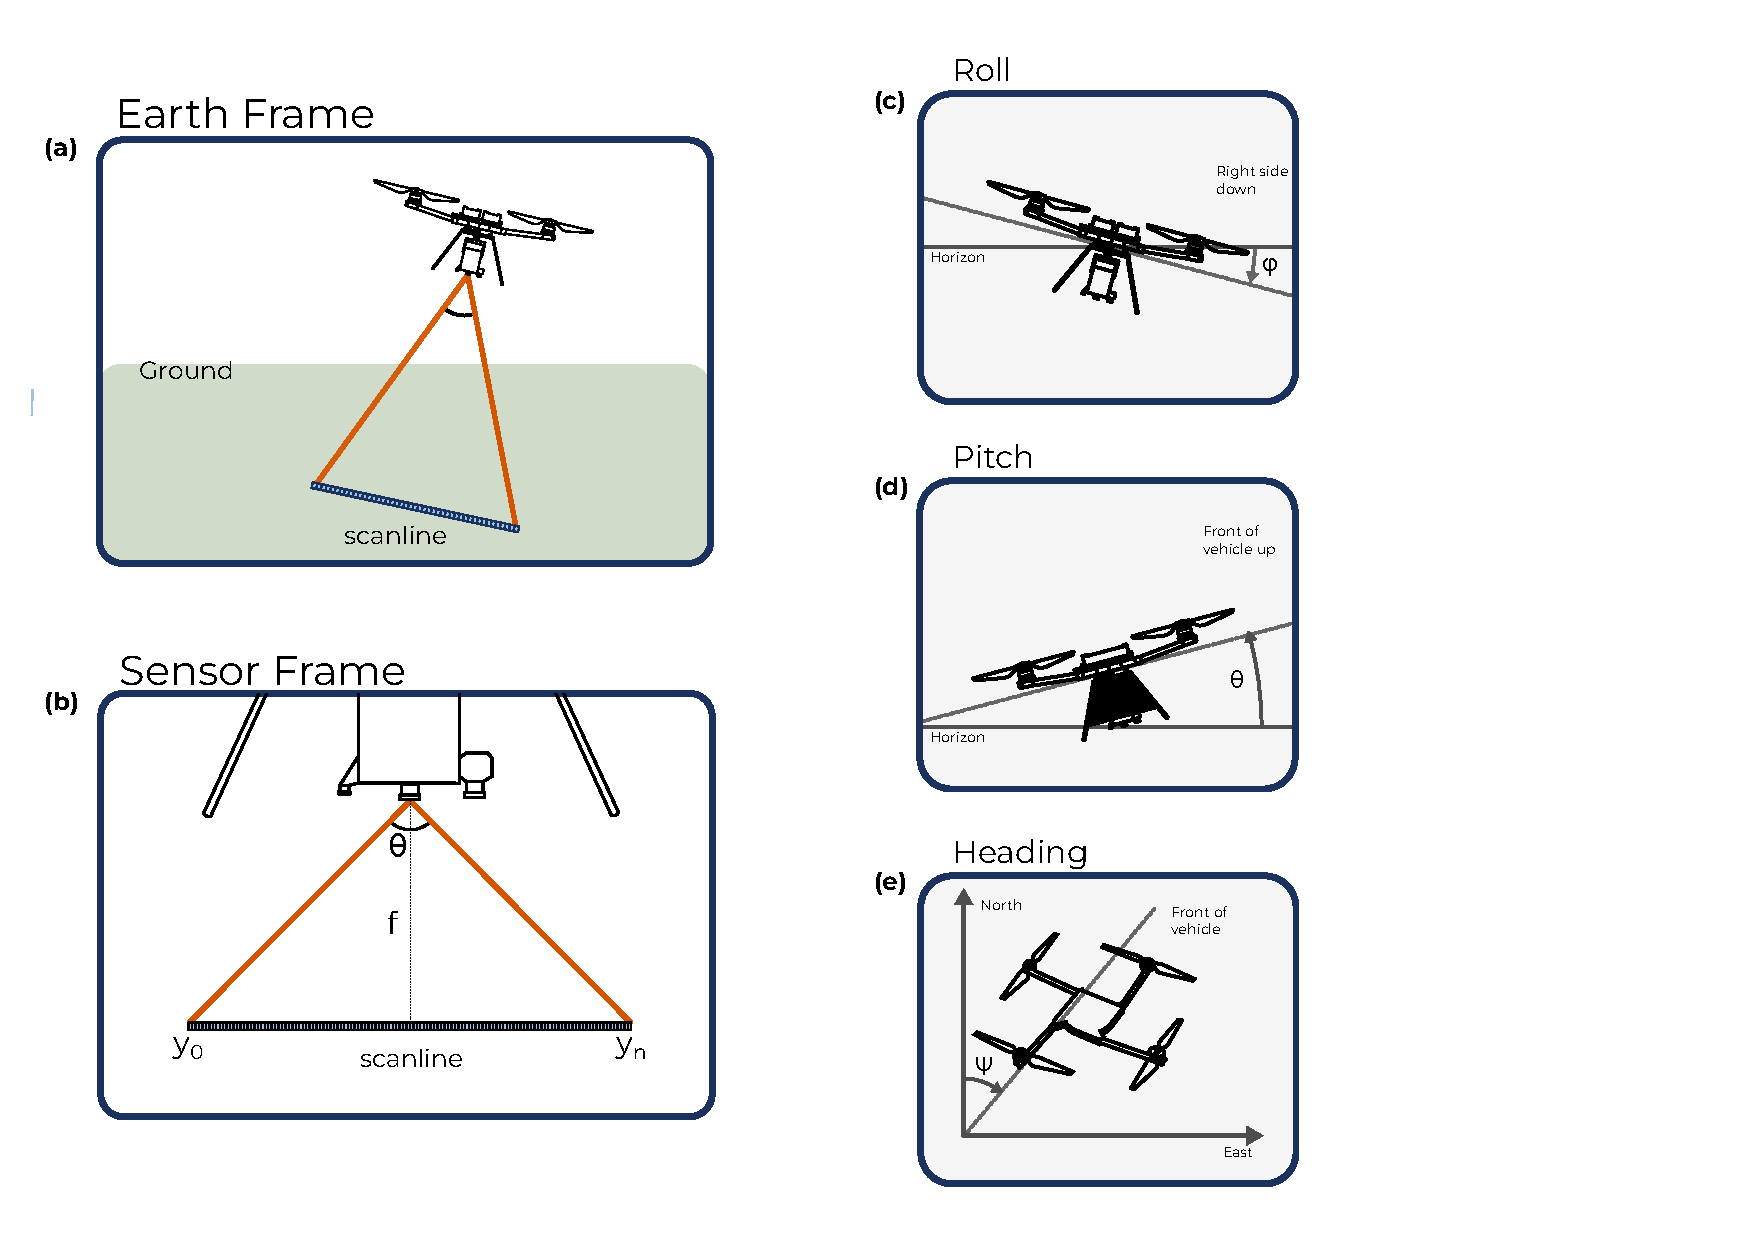
\includegraphics[width=0.95\columnwidth]{robot-team/georectification.pdf}
  \caption{Visual representation of sampling geometry for the UAV. (\textbf{a})
    the scan-line as seen from the Earth frame. (\text{b}) the HSI scan-line as
    represented in the frame of the sensor. (\textbf{d, d, e}) The angles
    describing the orientation of the drone in flight.}
  \label{fig:georectification}
\end{figure}

The GPS and IMU on the hyperspectral imager continuously capture the location $(\lambda,
\Phi, z)^T$  (longitude, latitude, altitude) of our drone as well it's
orientation defined by the angles $\phi$, $\theta$, and  $\psi$ (roll, pitch,
and heading). To georeference each pixel, we therefore must transform its
position from the frame of the sensor (measured in pixels relative to the
imager's sensor) first to the frame of the IMU used to measure the orientation,
then to the navigation frame (East, North, up), and finally to the ground frame. Let us
define the \textit{sensor} frame so that the scan-line falls upon the y axis. As
each scanline must be transformed independently, we can assign it an
x-coordinate of $0$ pixels. Lastly, if the viewing angle of the HSI is
$\theta_{\text{view}}$, then the coordinates of the i-th pixel,
$\mathbf{r}_i^{\text{sensor}}$, in the sensor frame are defined as in panel (b)
of Figure \ref{fig:georectification} to be
\begin{equation}
  \mathbf{r}_i^{\text{sensor}} = \left[ 0, y_i, f \right]^T
\end{equation}
where $y_i\in \left\{-\frac{(N-1)}{2},...,\frac{N-1}{2}\right\}$ and
$f=\frac{(N-1)/2}{\tan(\theta_{\text{view}}/2)}$ for $N$-total pixels per
scan-line. To align the sensor frame with the axes of
the IMU, we apply a sequence of rotation matrices defined using the measured
orientation angles (panels (c), (d), and (e) of Figure
\ref{fig:georectification}), denoted by
\begin{equation}
  \begin{aligned}
    &\mathbf{R}_{\text{sensor}}^{\text{IMU}}(\phi,\theta,\psi) = \\
    &\begin{bmatrix}
    \cos(\psi)\cos(\theta) & \cos(\psi)\sin(\theta)\sin(\phi)-\sin(\psi)\cos(\phi) & \cos(\psi)\sin(\theta)\cos(\phi)+\sin(\psi)\sin(\phi) \\
    \sin(\psi)\cos(\theta) & \sin(\psi)\sin(\theta)\sin(\phi)+\cos(\psi)\cos(\phi) & \sin(\psi)\sin(\theta)\cos(\phi)-\cos(\psi)\sin(\phi) \\
    -\sin(\theta) & \cos(\theta)\sin(\phi) & \cos(\theta)\cos(\phi)
     \end{bmatrix}.
  \end{aligned}
\end{equation}

Next, an orthogonal transformation is applied to transform from the IMU frame to
the navigation frame of the drone. This is important as the axes of the IMU and
the drone itself are not necessarily identical depending on how the IMU is
oriented on the HSI. For the UAV, this amounts to
\begin{equation}
  \mathbf{T}_{\text{IMU}}^{\text{DRONE}} = \begin{bmatrix}
    0 & 1 & 0 \\
    1 & 0 & 0 \\
    0 & 0 & -1
    \end{bmatrix}.
\end{equation}
At this stage, the pixel coordinates have been rotated into the frame of the
drone and must be rescaled from pixel units to meters. This is accomplished by
observing that panels (a) and (b) of Figure~\ref{fig:georectification} form
similar triangles with an shown in Figure~\ref{fig:s-geom}.

\begin{figure}[h]
  \centering
  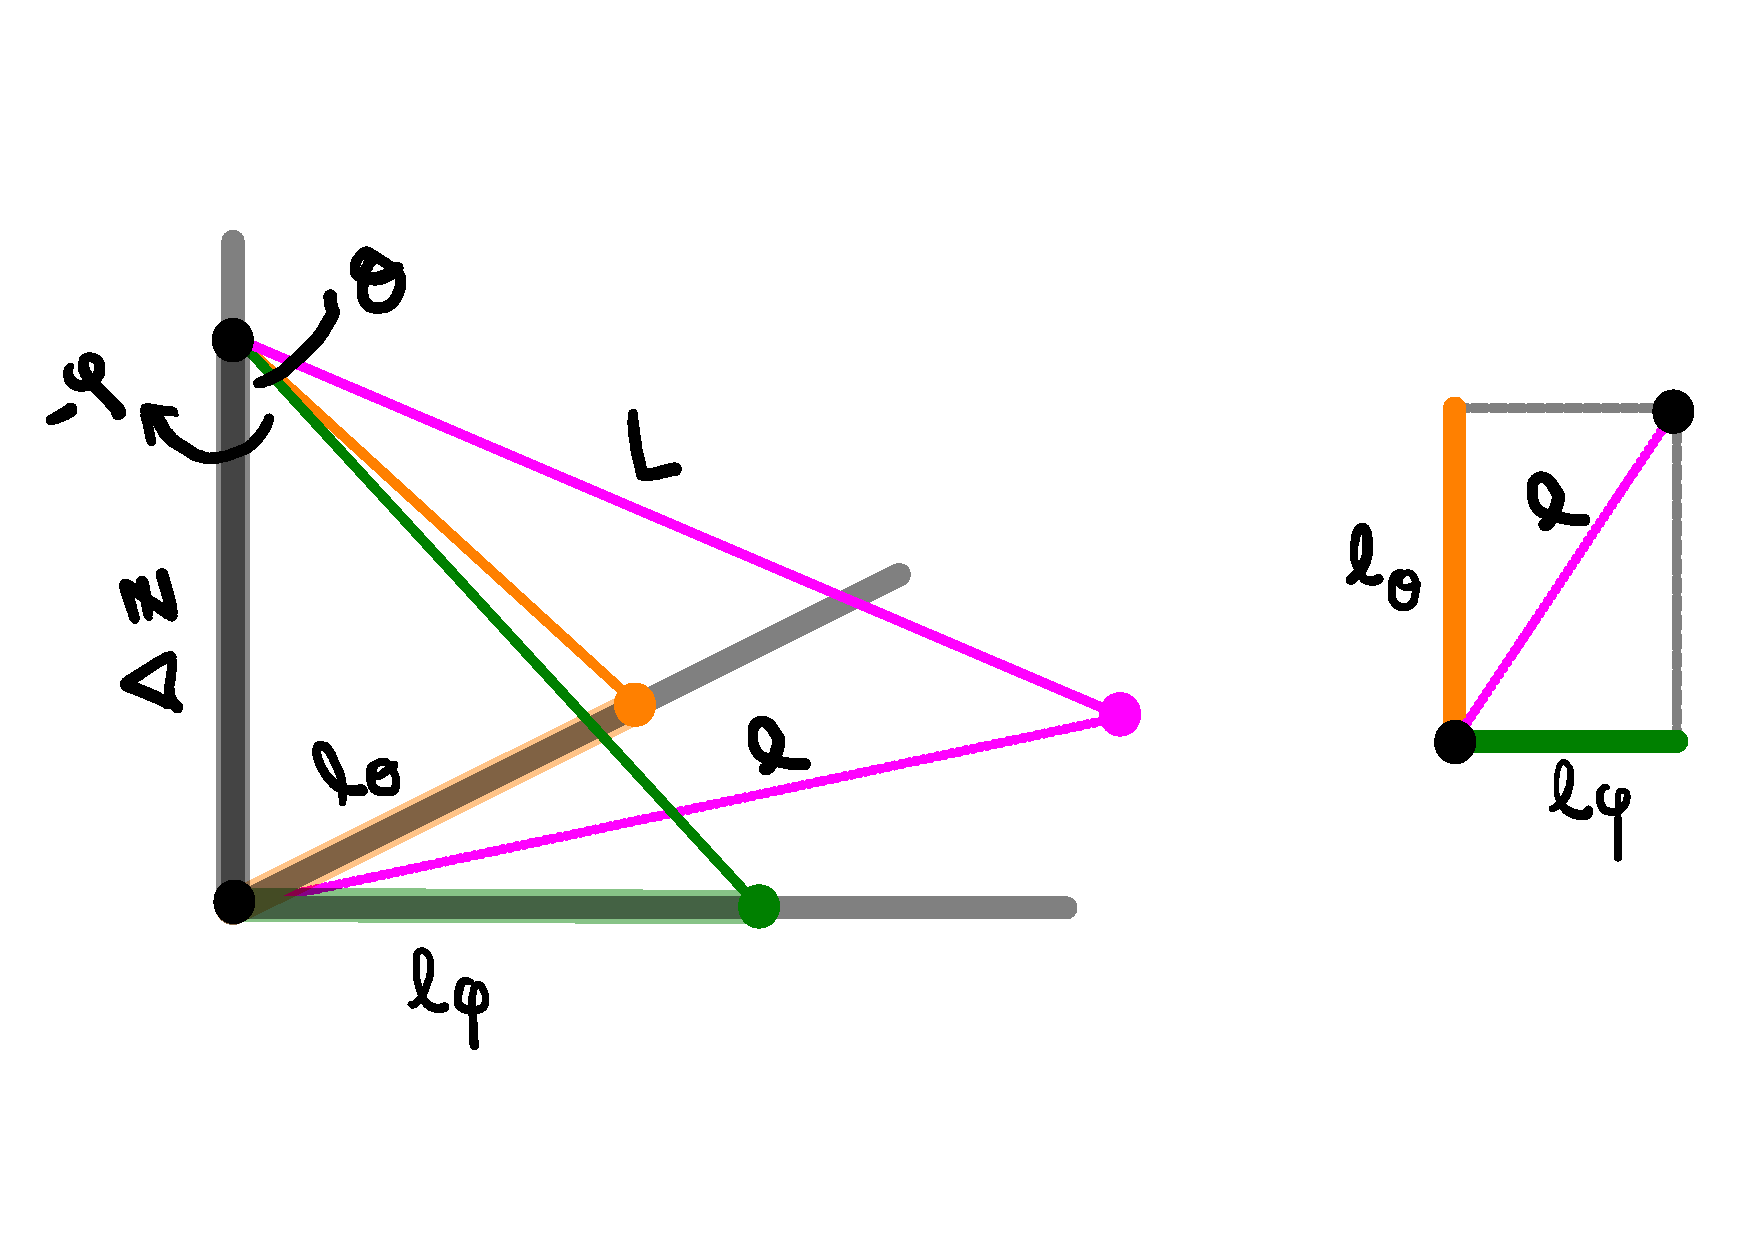
\includegraphics[width=0.6\columnwidth]{robot-team/scale-factor-geometry.pdf}
  \caption{At a height $\Delta z$, the position of an HSI pixel in the Earth
    frame depends on the roll $\theta$ and pitch $\phi$.}
  \label{fig:s-geom}
\end{figure}

For a height $\Delta z = z-z_{\text{ground}}$ above the ground, the distance $L$ from
the camera to an HSI pixel on the ground is
\begin{align*}
  L &= \sqrt{\Delta z^2 + \ell^2} \\
    &= \sqrt{\Delta z^2 + \Delta z^2\tan^2\theta + \Delta z^2\tan^2(-\phi)} \\
    &= \Delta z \sqrt{1 + \tan^2\theta + \tan^2\phi}
\end{align*}
leading to a scale factor
\begin{equation}
  s = \frac{L}{f} = \frac{\Delta z}{f}\sqrt{1 + \tan^2\theta + \tan^2\phi}.
\end{equation}

Finally, the coordinates of each pixel are translated using the position of the
drone in the chosen coordinate system. As the geometric transformations are
scaled to units of meters (by $s$), a coordinate transformation $f$ is applied to
obtain the position of the drone with respect to a local coordinate system such
as the Universal Transverse Mercator (UTM). Written all together, this becomes
\begin{equation}\label{eq:georec-eqn}
  \mathbf{r}_{i}^{\text{UTM}} =
  f_{\text{geo}}^{\text{UTM}}\begin{bmatrix}
    \lambda \\
    \Phi \\
    z_{\text{drone}}
  \end{bmatrix}_{\text{GPS}}^{\text{geo}} + s\mathbf{T}_{\text{IMU}}^{\text{DRONE}}\mathbf{R}_{\text{sensor}}^{\text{IMU}}(\theta, \phi, \psi)\begin{bmatrix}
    0 \\
    y_i \\
    f
  \end{bmatrix}^{\text{sensor}}
\end{equation}

The transformation from Equation~\ref{eq:georec-eqn} is applied \textit{in parallel}
to each scan-line to obtain the ground coordinates $\mathbf{r}_i=(x_i,
y_i,z_i)^T$ of each pixel. Finally, the resulting HSI is resampled to a
rectangular grid at a specified resolution by rounding each pixel's
coordinates to the desired accuracy and averaging all spectra that fall within the
same grid cell. Adjusting the final resolution of the georectified data cube
allows for optimization of compute time against spatial scale for real time
applications.

\subsection{Reflectance Conversion}

Once an HSI is georeferenced and resampled to the desired scale,
the downwelling irradiance spectrum measured during HSI acquisition is used to
convert the raw data from radiance to reflectance. This effectively normalizes
the HSI by \textit{dividing out} the incident light distribution making it possible
to compare spectra captured under variable lighting conditions. First,
the downwelling irraidance spectrum is loaded and interpolated to match the
wavelengths of the spectral bins of the hyperspectral imager. The reflectance at
pixel $(i,j)$ and wavelength $\lambda_k$ is then obtained by
\begin{equation}
  \rho_{ijk} = \frac{\pi L_{ijk}}{E_k}
\end{equation}
where $L_{ijk}$ denotes the original radiance pixel at wavelength bin $k$ and
$E_k$ denotes the downwelling irradiance at wavelength $\lambda_k$.

\begin{figure}[h]
  \vspace{-2cm}
  \centering
  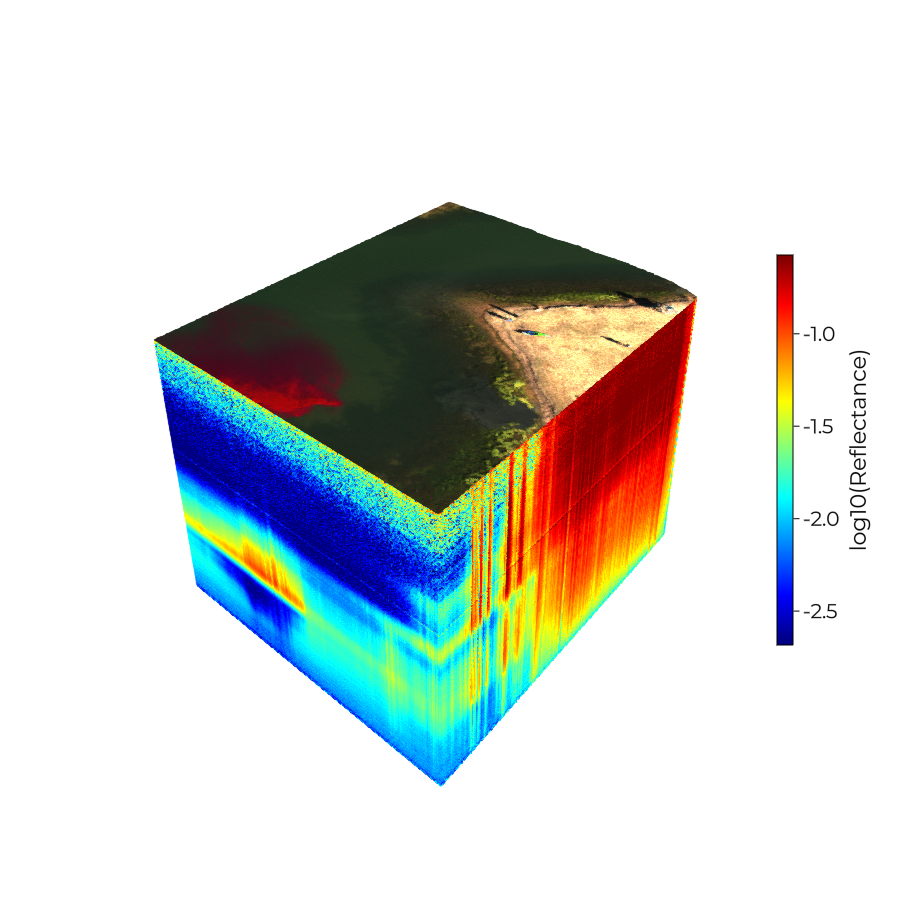
\includegraphics[width=0.55\columnwidth]{robot-team/georectification/demo-rectified-cube.png}
  \vspace{-1cm}
  \caption{Example of a georectified reflectance data cube. A pseudo color image is
    included at the top of the image showing what an observer would see from the
    perspective of the UAV. The log-10 reflectance is plotted at each wavelength
    bin along the z-axis. }
  \label{fig:sample-cube}
\end{figure}

Figure \ref{fig:sample-cube} illustrates an example of a georectified
reflectance data cube. The spectral signature corresponding to
a Rhodamine tracer dye released into the water is clearly visible in the front
left portion of the image.

\subsection{Timing Results}

This processing pipeline was implemented in the Julia programming language and
the associated code is accessible at \url{github.com/john-waczak/RobotTeam.jl}.
Using the package \texttt{BenchmarkTools.jl}, the time to load and georeference
HSI using the UAV processing computer for HSI with 371, 462, and 1000 scan-lines are
shown in Table~\ref{tab:georeference-times}.

\begin{table}[!hbt]
  \caption{Loading and georeferencing time as a function of number of scan-lines}
  \label{tab:georeference-times}
  \centering
  \begin{tabular}{cc}
    \hline
    \textbf{Number of scan lines}	& \textbf{Execution time (s)}\\
    \hline
    371		  &   0.161	\\
    462     &   0.197	\\
    1000    &   0.195  \\
    \hline
  \end{tabular}
\end{table}

The total processing time including resampling and conversion to reflectance as a
function of final resolution is shown in Figure~\ref{fig:regridding-timing} for
an HSI of initial size $1000\times 1600 \times 462$.

\begin{figure}[!hbt]
  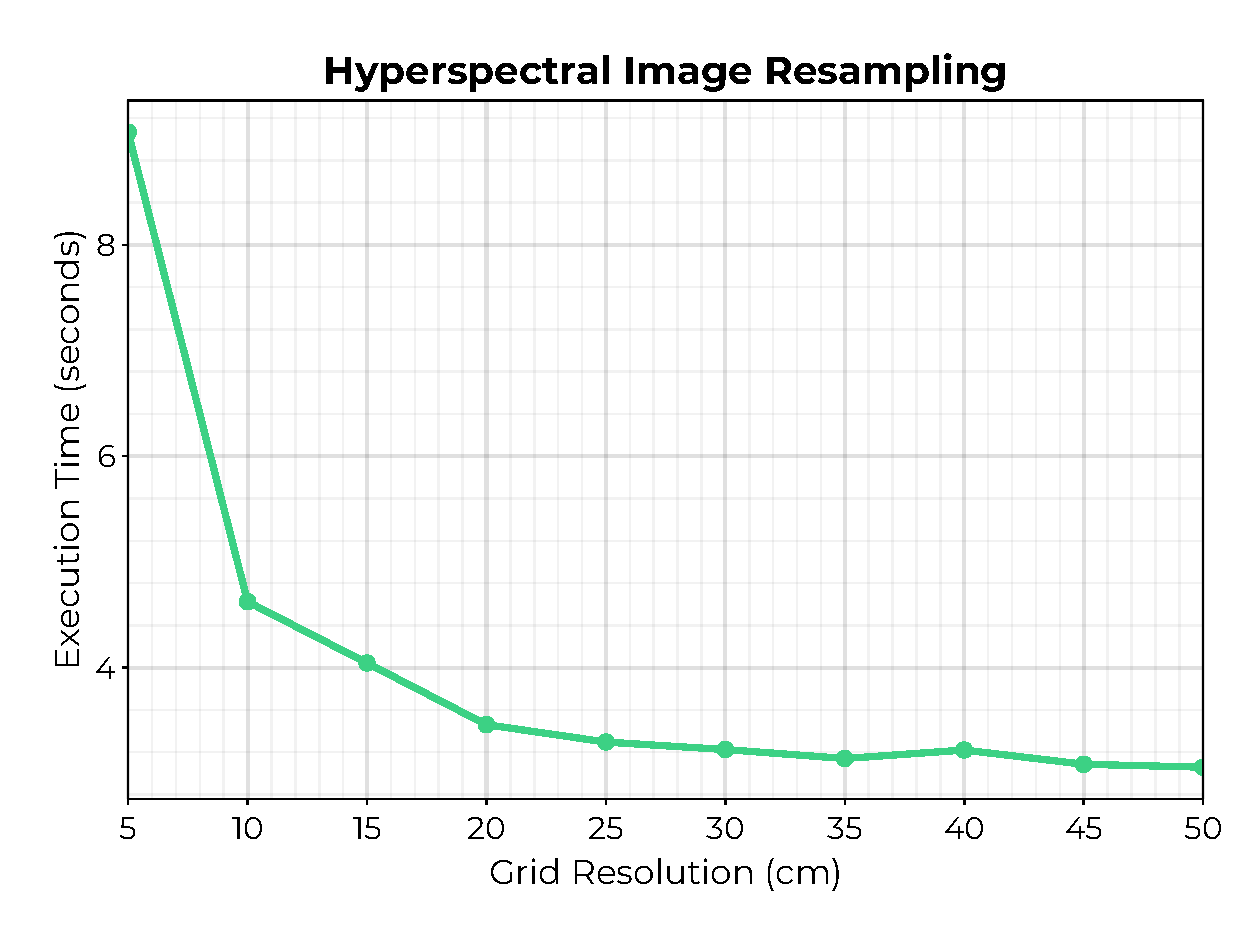
\includegraphics[width=0.85\columnwidth]{robot-team/georectification/regrid-timing.pdf}
  \caption{Timing results (in seconds) for resampling a 1000 scanline HSI as a function of output grid resolution.}
  \label{fig:regridding-timing}
\end{figure}

These timings indicate that processing an HSI to a final spatial resolution of
$20$ cm takes less than $4$ seconds which is comparable to the acquisition rate
of the hyperspectral imager. The key limitation of this implementation is the
assumption that the ground is flat. However, the studies in this dissertation
are focus specifically on imaging over the water where this approximation is
reasonable. For processing HSI collected over rough terrain, a digital elevation
map (DEM) can be used to augment the georectification process. Future iterations
of the drone can include small form-factor computers with integrated graphics
processing units (GPU) to accelerate these calculations. Here the problem of
georectification can be recast into a ray-tracing problem for each pixel
\cite{gpu-georect}.

\chapter{Distributed Sensor Networks for Real-Time Air Quality Assessment}\label{ch:air-network}

As outlined in Chapter~\ref{ch:intro}, air quality is a critical factor
affecting human health and well-being. Many pollutants such as Ozone, \ce{CO},
\ce{NO2}, \ce{SO2}, and volatile organic compounds contribute to poor air
quality. Among the variety of sources, particulate matter (PM) plays a
significant role and has
been linked to increased mortality by numerous studies
\cite{pm-mortality-six-cities, pm-mortality-2}. PM is particularly interesting
because its deleterious impacts on human health derive from both from its
composition \textit{and} its ability to penetrate into the tissues of the human
body. Beyond the obvious impact on lung health, PM pollution has been linked to
cardiovascular mortality \cite{pm-cardiovascular}, increased chronic kidney
disease \cite{pm-kidneys}, and recently, increased incidences of
neurodegenerative diseases like Alzheimer's \cite{pm-neurodegenerative,
  pm-neurodegenerative-2}. Therefore, the accurate assessment of PM exposure is
of paramount importance.

Considerable research efforts have focused on the development of accurate
measurement techniques for particulate matter. Unfortunately, most
reference-grade instruments remain prohibitively expensive, stunting our ability
to characterize spatial and temporal PM variations at scales relevant to dense
urban and suburban environments. Recently, a new class of low-cost PM sensors
based on optical particle counting has emerged. These sensors can be calibrated
against reference instruments using machine learning methods to improve
measurement accuracy and reduce inter-sensor variability
\cite{pm-calibration-lakitha}. Using these devices, our research group has
developed a family of low-cost monitors for real-time PM measurement. To date
over 100 monitors have been built and distributed across the Dallas Fort Worth
metroplex and other Texas cities.

In this chapter, we first describe physical measurement methods for PM. We then
describe the monitors developed by the MINTS research to provide real-time PM
measurements for a broad distribution of particle sizes. Finally, we describe
a comprehensive data pipeline developed for this dissertation which processes
real-time measurements measurement data and provides data visualization
dashboards. This system is designed using a variety of containerized open source
tools to guarantee reproducibility while ensuring the network can scale from
hundreds to thousands of sensors as they are built and deployed. Later
in Chapter~\ref{ch:havok} we analyze measurements collected
by sensors in this network to develop a physics-based method for outlier
detection and forecasting of PM time-series.

\section{Measurement of Particulate Matter}

Broadly speaking, instruments for measuring PM concentrations fall into one of
three categories:
\begin{itemize}
  \item \textbf{Federal Reference Methods} (FRM): These are methods which the US
    Environmental Protection Agency designate as the standard for PM measurement
    and may be used for assessing compliance with air quality regulations. The
    FRM for PM is \textit{gravimetric analysis} which collects size-selected
    particulate matter samples onto a polytetrafluoroethylene (PTFE) filter which are
    then carefully weighed to determine PM concentration by combining the sample
    mass with the sample flow rate \cite{pm-federal-reference-method}. Standard
    sizes are for PM 2.5 and PM 10 which correspond to particles with an
    aerodynamic diameter of $\leq 2.5$ $\mu m$ and $\leq 10$ $\mu m$, respectively.
  \item \textbf{Federal Equivalent Methods} (FEM): These measurement techniques
    include \textit{Beta Attenuation Monitors}  (BAM), \textit{Tapered Element
      Oscillating Ribbon} (TOEM) monitors, and \textit{Optical Particle
      Counters} (OPC) based on light scattering. FEM methods are also approved
    by the US EPA for ambient PM monitoring.
  \item \textbf{Low-cost Sensors}: These sensors are much less expensive than
    FRM and FEM systems but are not approved by the EPA for assessment of
    compliance with government regulations. Most low-cost sensors are simplified
    OPC systems.
\end{itemize}
The PM sensors described in this chapter fall into the low-cost OPC category.

\subsection{Optical Particle Counters}

Particulates scatter light according to their size and relevant physical
properties as described by Mie Scattering Theory for spherical dielectrics of
any radius. Optical particle
counters use light scattered off of particulates to estimate their size and
concentration. This method assumes particles are spherical and uses a
sufficiently slow flow rate so that, statistically speaking, particles enter the
sensing element individually. An example design for an OPC is shown below in
Figure~\ref{fig:opc-diagram}.

\begin{figure}[h]
  \centering
  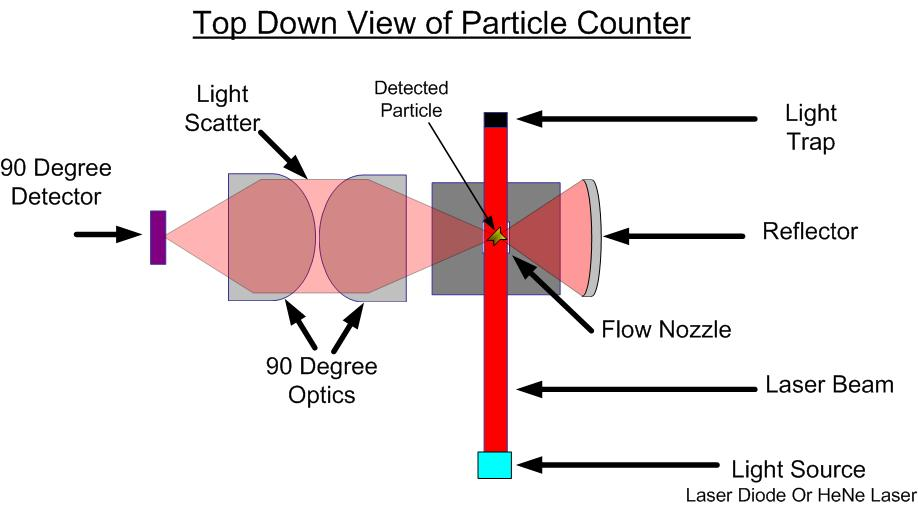
\includegraphics[width=0.7\columnwidth]{air-network/particle-counter.jpg}
  \caption{Optical particle counter: particulates are guided into the sensing
    element where a light source is then scattered off of the sample. This scattered
  light is then directed to detector. The inensity of scattered light is used to
distinguish particles by size. Image source: Morgan Polen, marked as public domain
(\url{https://en.wikipedia.org/wiki/File:Particlecounter.jpg}, accessed 2024-11-09). }
  \label{fig:opc-diagram}
\end{figure}

Particles are counted and sorted into distinct size bins based on the scattered
intensity with the detector oriented to limit the impact of index
of refraction on the scattered signal. For calibration,
most instruments use size-selected polystyrene spheres. Particle counts are then
converted into mass concentrations, for example PM 2.5 measured in $\mu g/m^3$.
This conversion is accomplished by assuming a constant particle density
consistent with observations for urban aerosols \cite{pm-density}.

An important consideration for OPCs is the impact of hygroscopic growth on
particle counts. When the humidity is sufficiently high, water tends to adsorb
onto particulates causing them to swell in size. Additionally, moistened
particulates may also agglomerate, coming together to form a larger particle
masses. This can significantly affect the accuracy of PM measurements by OPCs
leading to distortions in the estimated size distribution causing overestimation
of the true particulate mass. For this reason, FEM instruments using the OPC method
often include humidity control and heating elements. This significantly improves
the accuracy of sensor measurements but decreases the sampling rate to $1-10$
minutes per reading and increasing power consumption and instrument cost.
With the growing interest in low-cost OPC-based sensors, a variety of
corrections using local temperature and humidity data have also been suggested
\cite{opc-corrections}.

The current iteration of air quality monitors designed by the MINTS research
group utilize the Pierra Systems IPS7100 Intelligent Particle Sensor. This
device is capable of measuring PM concentrations at 1 Hz across 7 size bins
enabling concentration measurements for PM $0.1$, $0.3$, $0.5$, $1$, $2.5$, $5$,
and $10$. Estimation of ultra-fine particulates is made possible due to the
detectors $1$ MHz sampling rate. We note that the $0.1$ $\mu m$ size bin, is
extrapolated from the measured size distribution. An example of an individual
IPS7100 sensor is shown in Figure~\ref{fig:ips7100}.

\begin{figure}[!h]
  \vspace{-1cm}
  \centering
  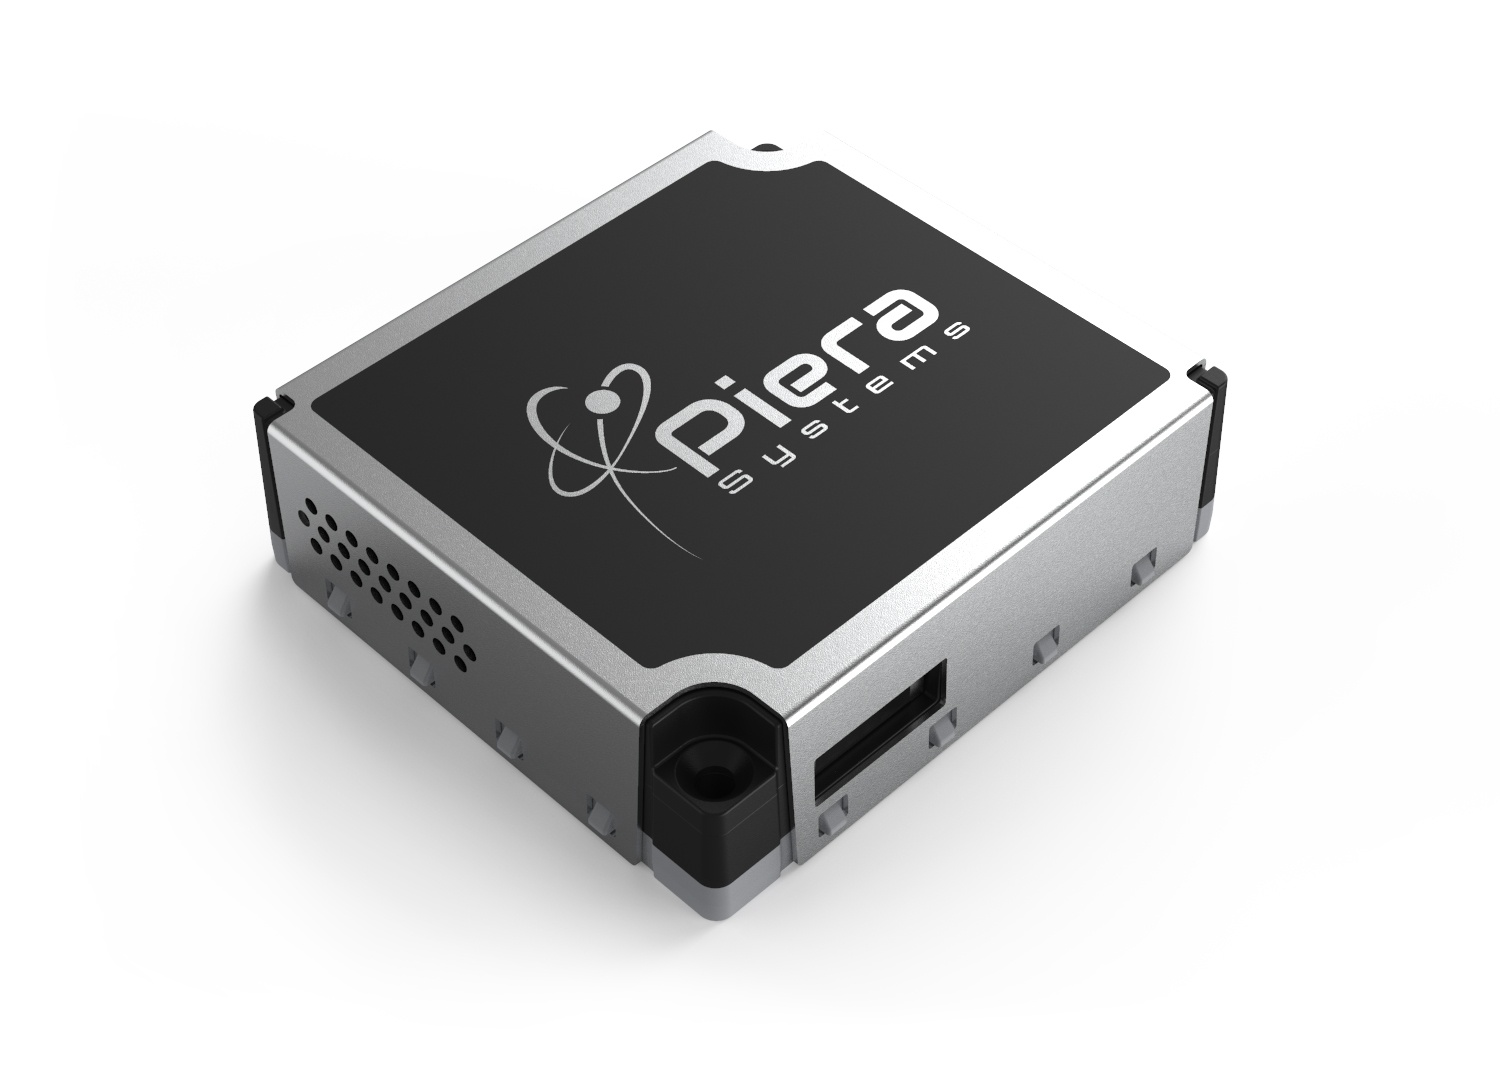
\includegraphics[width=0.4\columnwidth]{air-network/ips7100.jpg}
  \caption{The Pierra Systems IPS7100 Particulate Sensor.}
  \label{fig:ips7100}
\end{figure}

\section{A Low Cost Sensor Network For Air Quality Monitoring}


% The highly expensive cost to acquire, calibrate, and maintain reference grade
% air quality monitors makes it challenging to assess the importance of spatial
% and temporal variability on local air quality. Since factors such as weather,
% terrain, traffic, and the distribution of other sources can all effect local air
% quality, the development of low-cost sensing solutions is vital to address risks
% of poor air quality on local communities. To address this gap, we have developed
% a hierarchy of low-cost air quality monitors which we have deployed throughout
% the Dallas Fort-Worth (DFW) metroplex. In this section, we describe the relevant
% sensor types as well as a robust data processing and visualization pipeline
% developed to enable open access to high quality data.

\subsection{Sensor Nodes}

The sensor network is comprised of a combination of two types of nodes:
\textit{Central Nodes} and \textit{LoRa Nodes}. The central nodes are designed
to be deployed in locations with where dedicated power is available. Each
contains a variety of sensors including the IPS7100, VOCs,
\ce{CO2}, \ce{NO_X}, ionizing radiation, incident light intensity,
sound levels, as well as meteorological variables including temperature,
pressure, relative humidity, and dew point. The powered Central Nodes are
equipped with a cellular modem to facilitate data transfer from the field.


Each Central Node supports a collection of ~10 LoRa nodes (named for the
long rage wireless transmission protocol) which can be separated by distances up
to ~5 km or more if line of sight is established. These smaller sensors are self
powered using a combination of battery and solar cells, and each measures a
similar assortment of air quality parameters including particulate matter
concentrations, gas concentrations, and meteorological parameters. Designs for
the two node types are illustrated in Figure~\ref{fig:mints-nodes}.

\begin{figure}[!hbt]
  \begin{subfigure}{.5\textwidth}
    \centering
    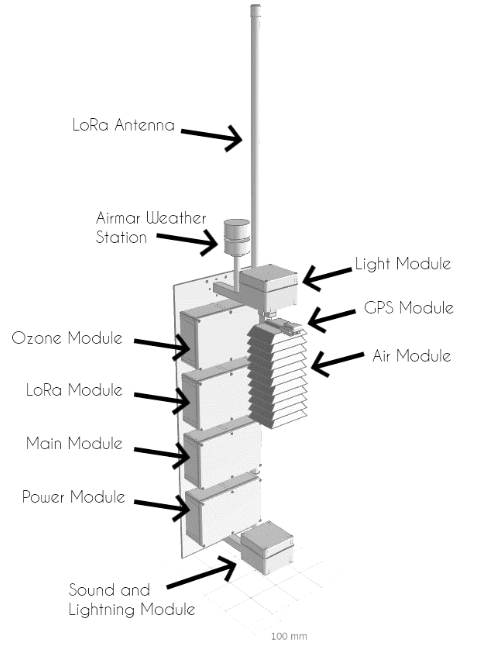
\includegraphics[width=.8\linewidth]{air-network/central-node.png}
    \caption{A 3d model of a Central Node}
  \end{subfigure}
  \begin{subfigure}{.5\textwidth}
    \centering
    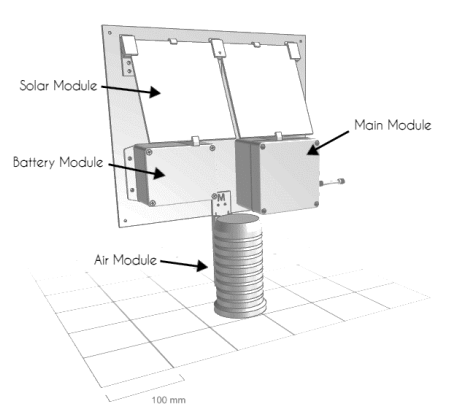
\includegraphics[width=.8\linewidth]{air-network/lora-node.png}
    \caption{A 3d model of a LoRa Node}
  \end{subfigure}
  \caption{Two types of nodes from the MINTS Air Quality network. Reproduced
    with permission from \cite{lakitha-thesis}}
  \label{fig:mints-nodes}
\end{figure}

Using the LoRaWAN protocol, Central and LoRa nodes form a low-power, wide-area
network through which data packets containing live measurements from each
LoRa node are transmitted to the nearest Central Node. The central nodes then
pass measurement data to a to a data processing backend using an MQTT
publish-subscribe model with their build-in cellular connection \cite{mqtt}.
Beginning in 2020, the first generation of nodes were built and installed as
shown in Figure~\ref{fig:sharedair-site}. In addition to sensor from MINTS, the
map also shows EPA reference sensors as well as live sensors from the PurpleAir network.

\begin{figure}[!hbt]
  \centering
  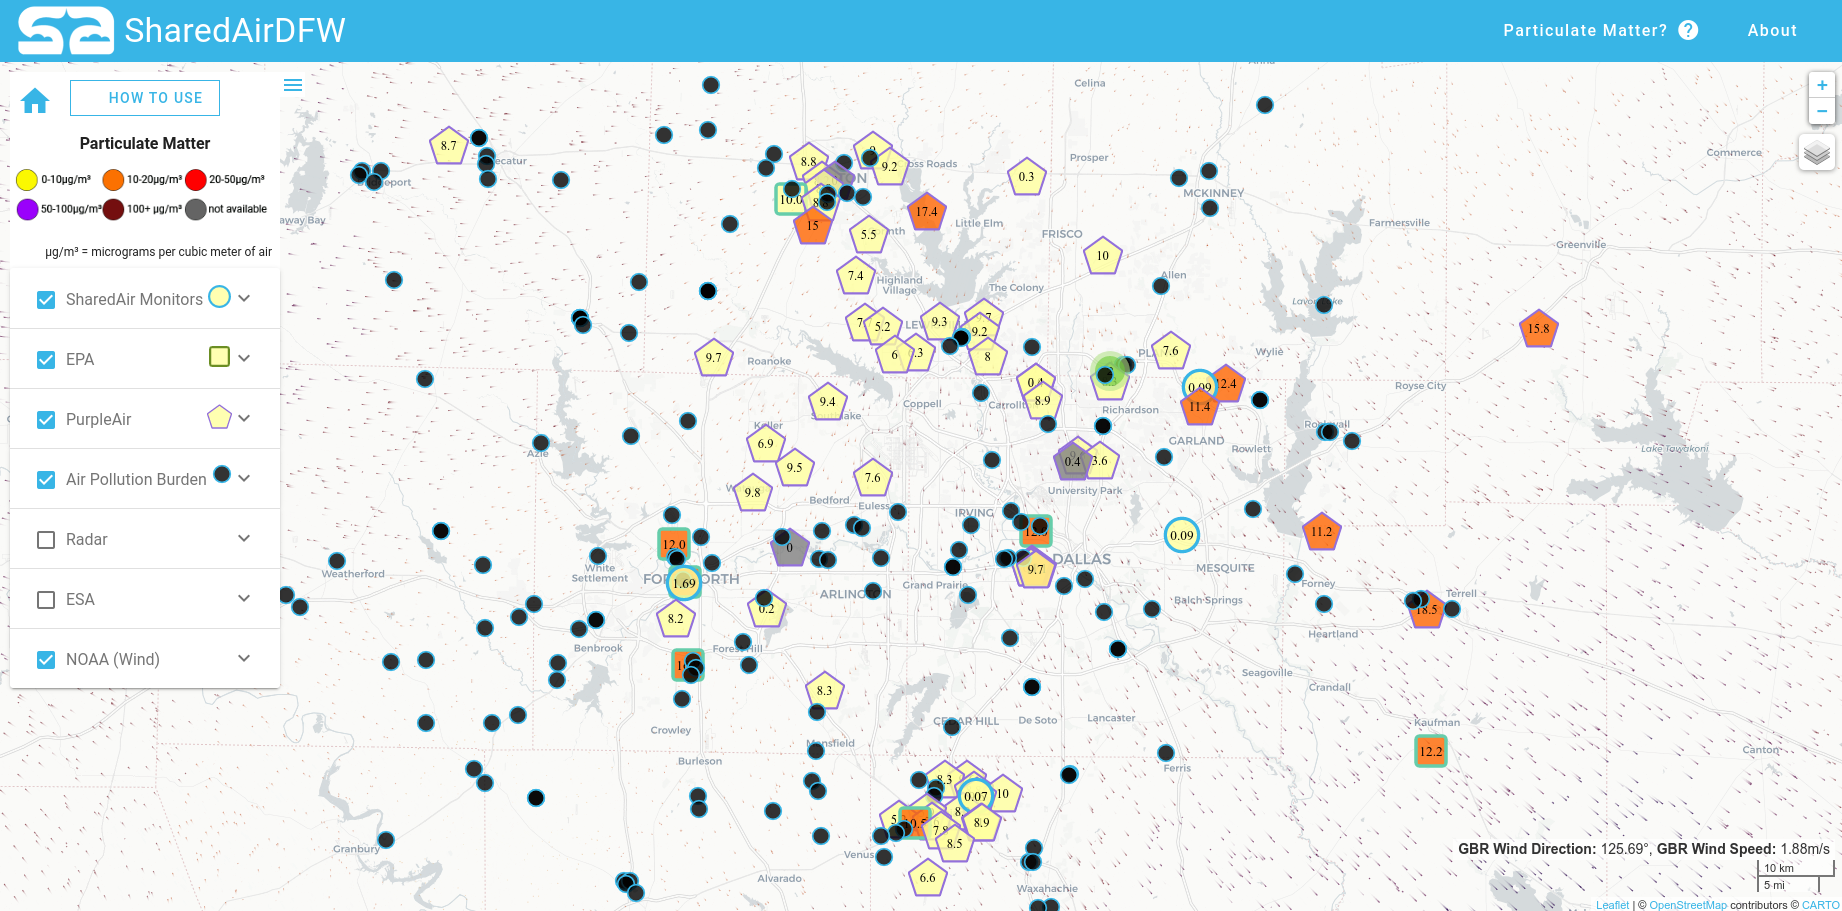
\includegraphics[width=0.85\columnwidth]{air-network/sharedairdfw-homepage.png}
  \caption{Interactive website displaying live sensor data on map. MINTS sensors
  are denoted with circular markers and additional data sources from EPA
  monitoring sites and PurpleAir monitors are included. Wind fields visualized
  using forecasts provided by NOAA.}
  \label{fig:sharedair-site}
\end{figure}


\subsection{The Data Pipeline}

To make real-time data available for public consumption and further analyses, a
containerized pipeline was implemented which combines a variety of open-source
data processing and visualization tools. \textit{Containerization} is a
method of encapsulating software together with
all of its dependencies, libraries, and configuration settings. Critically,
containerization makes software components such as databases and web servers
highly portable so that tools can be developed locally and then deployed to
remote systems.

Containers are defined using \textit{Dockerfiles} and can be networked together
with common data storage to achieve complex workflows. The pipeline developed
for the MINTS air quality network combines three containerized open-source tools:
\begin{itemize}
\item \textbf{NodeRed}: This tool developed by IBM allows the creation of
  data processing pipelines by defining directed acyclic graphs (DAGs)
  composed of individual processing nodes. This tool is utilized to subscribe to
  each sensor's MQTT topics and decode binary data packets into individual
  sensor measurements. Processed data are then injected by NodeRed into a
  time-series database. A key advantage of NodeRed is that the vast set of
  pre-implemented nodes which provde an easily maintainable, low-code data
  processing environment.
\item \textbf{InfluxDB}: This is a open source time-series database optimized
  for large cardinality datasets. By storing processed data in InfluxDB, we are
  able to provide queryable access to live and historic measurements.
\item \textbf{Grafana}: This tool is an visualization platform for
  creating interactive dashboards. Grafana is connected to InfluxDB to provide
  detailed, real-time displays for each sensor in the network. These dashboards
  visualize data from \textit{all} incoming measurements from each node in
  addition to the PM.
\end{itemize}

\begin{figure}[!h]
  \centering
  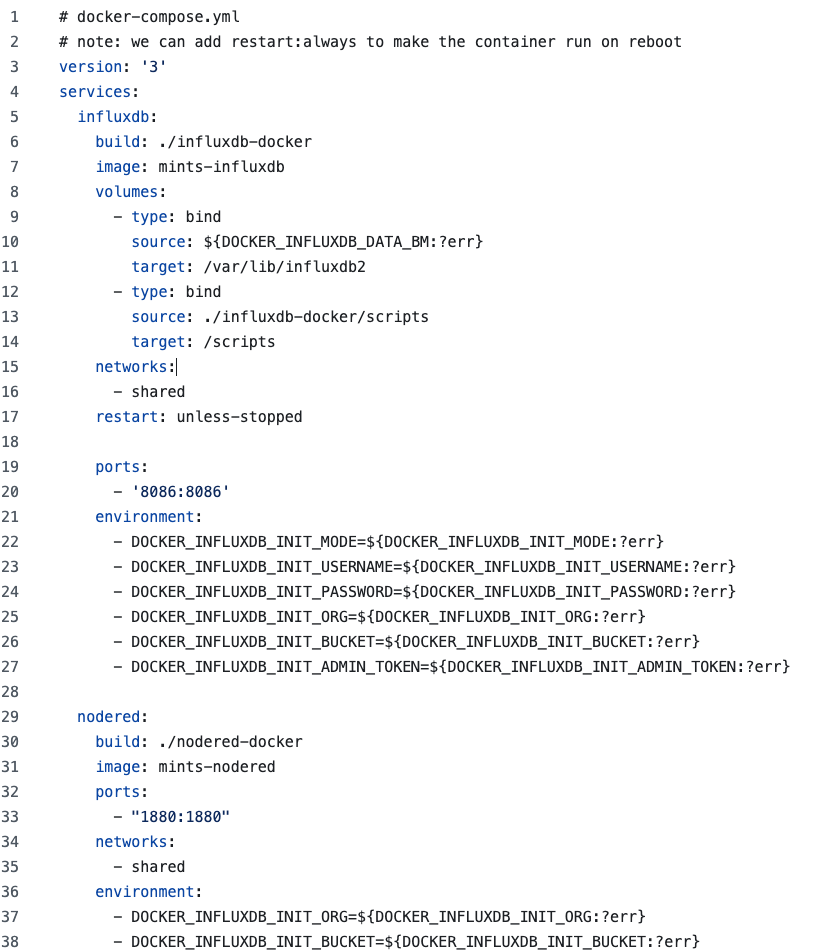
\includegraphics[width=0.95\columnwidth]{air-network/compose-snippet.png}
  \caption{Snippet of the \texttt{docker-compose.yml} file showing the
    combination of InfluxDB and NodeRed. Each individual container can define
    network ports, shared data volumes, and environment variables.}
  \label{fig:compose}
\end{figure}

Container orchestration is accomplished using YAML files like the examples shown
in Figure~\ref{fig:compose}




\begin{figure}[!h]
  \centering
  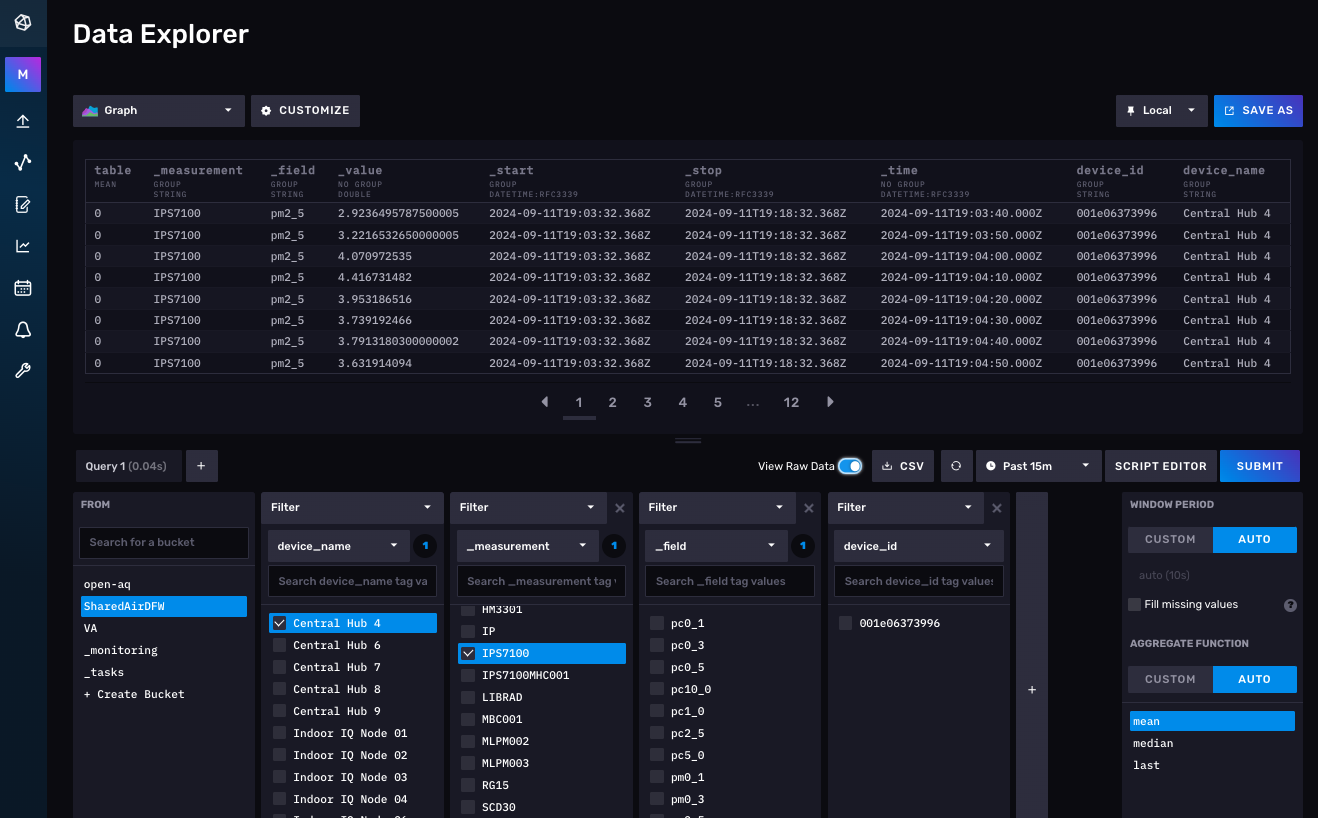
\includegraphics[width=0.95\columnwidth]{air-network/influxdb.png}
  \caption{A view of the time series data accessible from the InfluxDB database.
  Each sensor is assigned a unique device name. Time-series for individual
  sensor measurements can be identified by the sensor name and the specific
  measurement.}
  \label{fig:influxdb}
\end{figure}




\begin{figure}[!h]
  \centering
  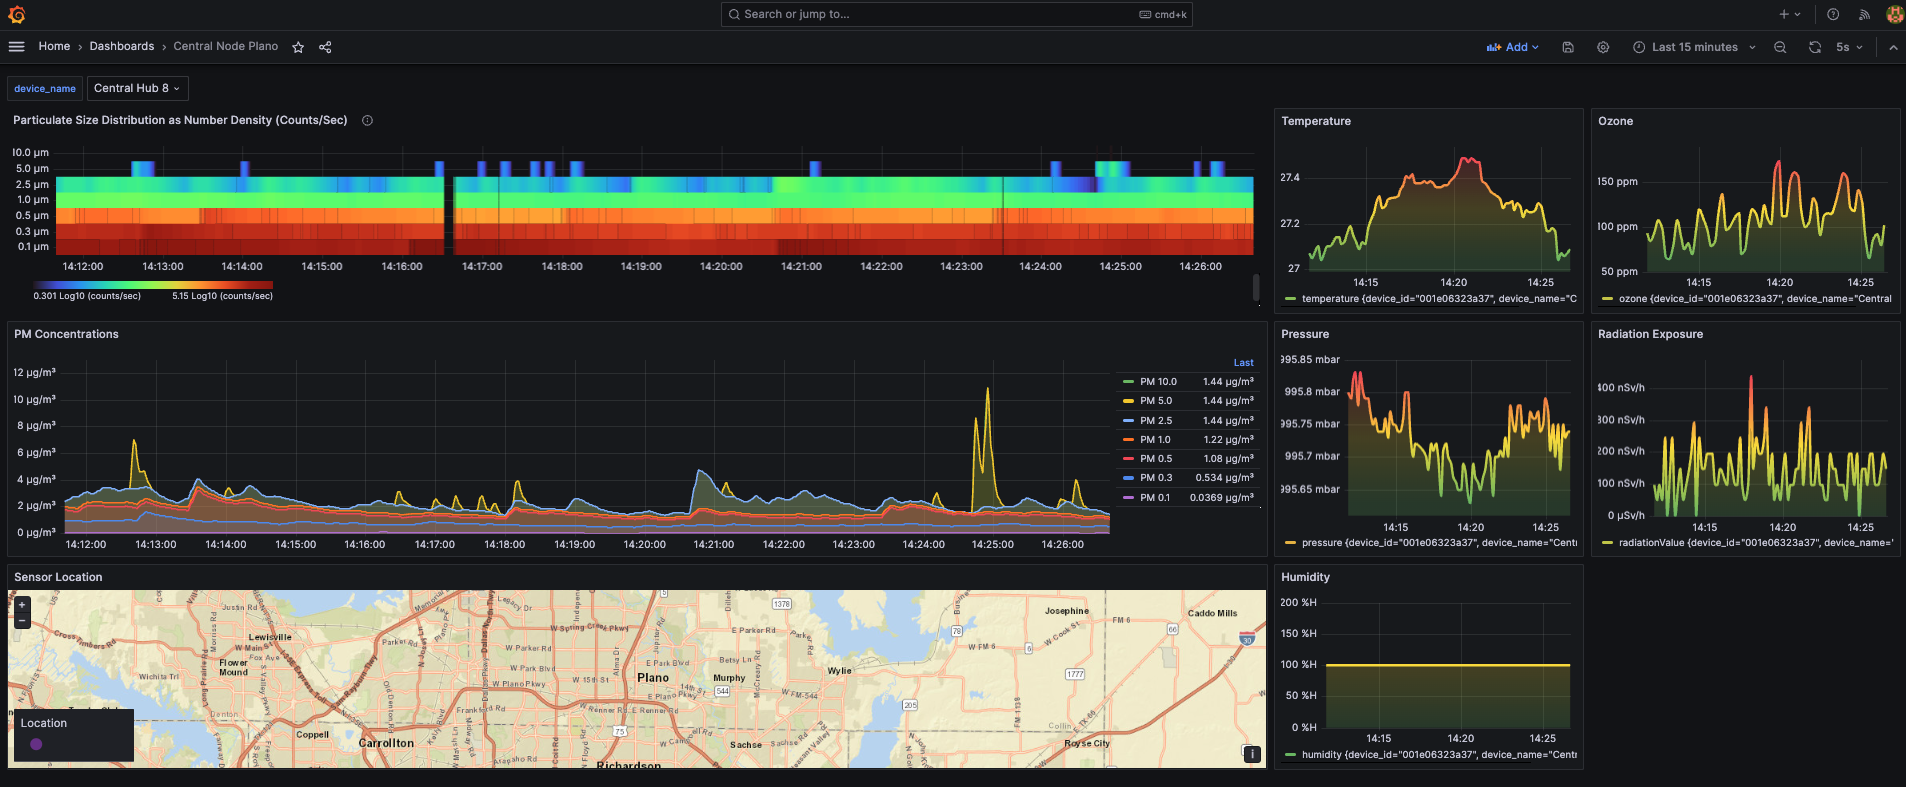
\includegraphics[width=0.95\columnwidth]{air-network/grafana.png}
  \caption{Example grafana dashboard}
  \label{fig:grafana}
\end{figure}





\textbf{Open Storage Network}: With help from Dr. Chris Simmons, we have
  developed a pipeline for long term data storage utilizing the Open Storage
  Network to provide open access to historic sensor data stored in the popular
  S3 format.
 



\chapter{A Chemical Data Assimilation Framework for Indoor Air Quality Assessment}\label{ch:autochem}


\section{Gaussian Processes}

\section{Adjoint Methods for Optimization}
\subsection{Linear Systems}
\subsection{Nonlinear Systems}
\subsection{Ordinary Differential Equations}


\section{Data Assimilation}
\subsection{Kalman Filter}
\subsection{Extended Kalman Filter}
\subsection{Continuous-discrete Extended Kalman Filter}
\subsection{3d-Var}
\subsection{4d-Var}

\section{Physics of Chemical Reactions: Chemical Reaction Kinetics}
\subsection{Overview}
\subsection{Chemical Equilibrium and the Law of Mass Action}
\subsection{Reaction Rate Laws}

\section{Summary of Chemical Mechanism Kinetics}

\section{Characterization of Photolysis Rates}
\subsection{Absorption Cross Sectionss}
\subsection{Quantum Yields}
\subsection{Photolysis Rate Determination}

\section{Chemical Data Assimilation}

\section{Results}

\section{Discussion}

\chapter{Future Work}\label{ch:future-work}

\section{Robot Team}

Minaturization of drones - next generation hyperspectral imagers (smaller) on smaller drones with additional payloads for visible and thermal imagers (not previously utilized)

Multi-sensor fusion and super resolution, e.g. use fine spatial resultion of visible imager together with spectral resolution of HSI and thermal to create a blended data product

Combine drone based imaging with remote sensing hyperspectral data, e.g. Enmap, PACE, etc...

Drone swarms for faster data collection

Additional data collection (can we test the generalizability across water bodies)

Additional ions with application to battery stuff...

\section{GTM}

GTM for guided data collection viat prize-collecting travelling salesman problem.

GTM for dust source identification. We can encourage finer cluserting behavior by augmenting the GTM to use adaptive mixing coefficients $\pi_k$ as we did for the GSM.

Batch version implementation of the GTM for \textit{big} datasets and online learning.

\section{GSM}

GSM for algal bloom identifiaction using remotely sensed hyperspectral imagery.

GSM for source apportionment of air quality measurements

Batch version of the GSM for \textit{big} dtaasets.


\section{PM Modeling}

Using HAVOK model to automatically identify pollution events and generate short term predictions near real time.

\section{Air Parcel Back Trajectories}

Compute back trajectories of PM data using meteorological analysis (and re-analyses).

Applications to human health outcomes: Alzheimers


\section{Chemical Data Assimilation}

Air quality chamber.






\chapter{Conclusions}\label{ch:conclusions}

\textcolor{red}{\textbf{Robot Team Supervised:}}
In this study, we address two key limitations of current remote sensing
approaches to characterize water quality: namely, the limited spatial, spectral,
and temporal resolution provided by existing satellite platforms and the lack of
comprehensive in situ measurements needed to validate remote sensing data
products. By equipping an autonomous USV with a suite of reference sensors, we
rapidly collect significantly more data than existing approaches that rely on
the collection of individual samples for lab analysis or are constrained to
continuous sensing at fixed sites. Utilizing an autonomous UAV equipped with a
hyperspectral imager in tandem with the USV allows us to quickly generate
aligned datasets that are used to train machine learning models mapping measured
reflectance spectra to the desired water quality variables. By virtue of this
increased data volume, we are able to simultaneously estimate the uncertainty of
our models by using conformal prediction. Finally, the hyperspectral data cube
processing workflow employed onboard the UAV makes it possible to deploy these
trained models to swiftly generate maps of the target variables across bodies of
water. The rapid turnaround time from data collection to model deployment is
critical for real-time water quality evaluation and risk assessment.




\textcolor{red}{\textbf{Robot Team GTM}}
In this study, we present  GTM as a useful unsupervised method for the visualization of UAV-based hyperspectral imagery and associated extraction of spectral endmembers. Using data collected at a North Texas pond, we demonstrate how the latent space of the GTM can be used to visualize the distribution of observed reflectance spectra revealing the small-scale spatial variability of water composition. Spectral signatures extracted from GTM nodes are used to successfully map the abundance of algae near the shore and to track the evolution of a rhodamine tracer dye plume. These examples illustrate the power of combining unsupervised learning with UAV-based hyperspectral imaging for the characterization of water composition. Future work will further develop the GTM as a tool to guide in situ data collection and enable contaminant localization for real-time applications.




\appendix % required only if you have appendixes

%% \chapter{Reproducible Research Techniques}
\textcolor{red}{\textbf{UPDATE REQUIRED!}}

\section{Environment Management in Julia}
\section{Version Control (git)}
\section{CI/CD with github worfklows}
discuss automated tests as well as automatic document generation here

\section{Literate Programming and Automatic Documentation with Quarto}
\section{Containerization with Docker and Docker Compose}
Discuss NodeRed, InfluxDB, Grafana, etc...


%% \chapter{Optimization Methods}

Describe standard gradient descent and it's utility for machine learning. Expand to briefly describe the extensions used in our work:
\begin{itemize}
\item Gradient Descent
\item Gradient Descent with Momentum
\item ADAM
\item BFGS
\item LBFGS
\item The method we used for the variogram method that works specifically for quadratic loss functions...
\end{itemize}

We should also comment on which particular methods are best (and when)


%% \chapter{High Performance Computing}


Provide an overview of relevant concepts in high performance computing i.e.
\begin{itemize}
\item slurm
\item multi-threading
\item parallelization (distribured computing)
\item Memory management (i.e. preallocating data containers and writing functions that mutate, not allocate)
\end{itemize}


%% \chapter{A Chemical Data Assimilation Framework for Indoor Air Quality}




\section{Physics of Chemical Reactions: Chemical Reaction Kinetics}

\subsection{Overview}

Since the early successes of Newton's descriptions of mechanics by means of simple forces acting on masses, scientists have sought to understand the dynamics of chemical reactions in terms of the detailed microphysics of molecular collisions. As we shall see, this approach can be utilized productively to justify the complicated temperature and pressure dependence of the reaction rate coefficients of many elementary reaction. However, even when considering the asymmetric structure of many molecules, and therefore, the dependence on orientation at the collision site, kinetic theory alone is unable to model reaction rates in all relevant temperature and pressure regimes. To do this, one can utilize the modern treatment of \textit{Potential Energy Surface} (PES) theory together with the notion of short-lived, unstable intermediate reaction states to calculate reaction rate coefficient functions for specific reactants. \textit{Ab initio} solution of the Schrodinger equation for the relevant nuclear geometries ($3N$ reaction coordinates for $N$ atoms) together with scattering and spectroscopic methods as suggested by \cite{transition-state-spectroscopy-bimol} have led to significant improvements in our understanding of reaction dynamics.



\begin{figure}[h]
  \centering
  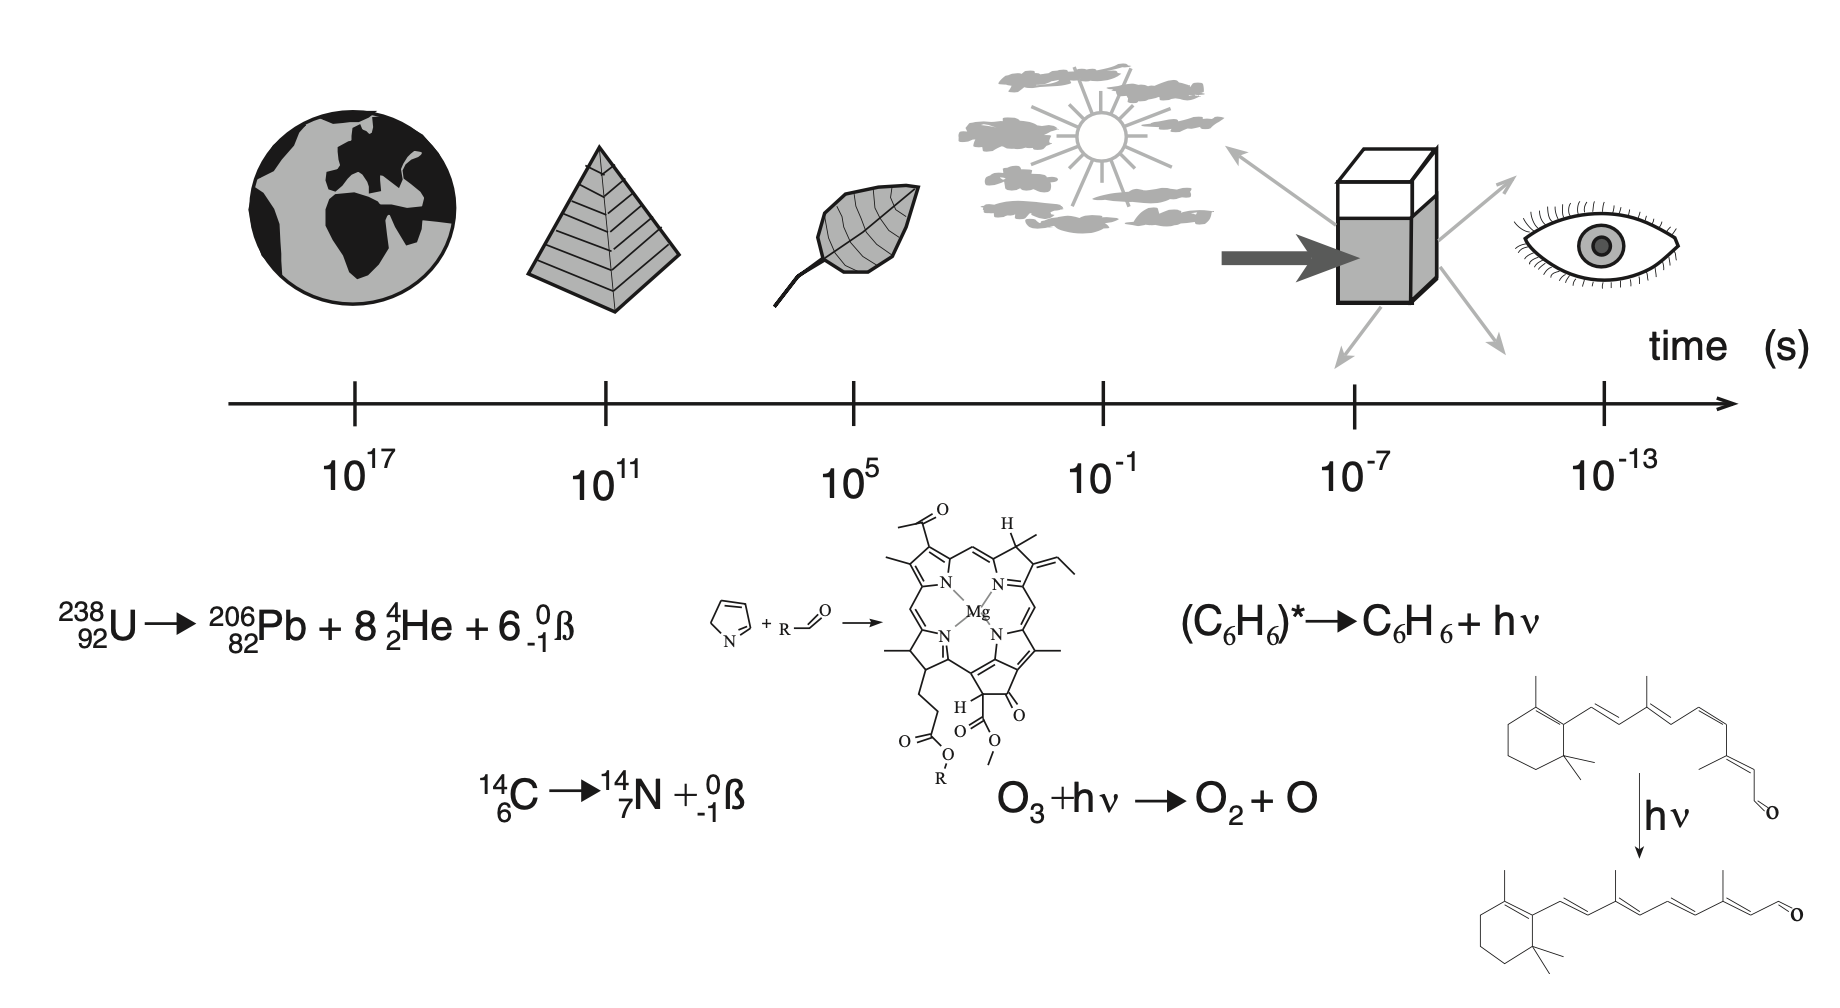
\includegraphics[width=0.85\textwidth]{introduction/reaction-timescales.png}
  \caption{An illustration of the broad range of reaction time scales from the long-lived nuclear decay to rapid degradation of molecules by photolysis. Figure taken from \cite{arnaut2006chemical}}
  \label{fig:reaction-timescales}
\end{figure}


However the computational complexity of this task makes it prohibitively expensive to perform at the scale required for our desired chemical mechanism which consists of many hundreds to thousands of reactants together with as many as 16,000 unique reactions. Therefore in the following discussion, we shall primarily utilize the kinetic theory to justify the functional form for \textit{most} rate coefficients with some reference to the extensions made by PES theory. We note that in practice, kinetic evaluations such as the periodic reports from the NASA Jet Propulsion Laboratory \cite{jpl-kinetic-evaluation-2020} utilize (justified) empirical fits to provide suggested functional forms for reaction rate coefficients.

\subsection{Chemical Equilibrium and the Law of Mass Action}

Before outlining the dynamics involved during complex chains of chemical reactions, it is worth spending some time to consider how we should treat chemical equilibrium. Usually in these scenarios we can not hold the internal energy fixed due to interactions with the environment, but rather, the temperature and pressure can often be treated as so. For example, we may be interested in gas-phase reactions occurring in ambient indoor air at or near standard temperature and pressure. In such scenarios, one finds the relevant potential energy to be the Gibbs, given by
\begin{equation}
  G = U - TS + PV,
\end{equation}
which is minimized in equilibrium under constant temperature and pressure.

This equation leads to the convenient thermodynamic identity
\begin{equation}
  dG = -SdT + VdP + \sum_i \mu_i dN_i
\end{equation}
from which we may identify the \textit{chemical potential} of the $i^{th}$ species as
\begin{equation}
  \mu_i  = \left(\frac{\partial G}{\partial N_i} \right)_{T,P,N_{j\neq i}}.
\end{equation}
The fact that each $\mu_i$ depends only on intensive state variables allows us to further simplify the relationship by considering what would happen were we to gradually increase the size of the system while maintaining the values of intensive parameters $T$, $P$, $\mu_i$. The result is G must increase in direct proportion to the increase in each $N_i$, that is:
\begin{equation}
  \label{eq:free-energy-definition}
  G = \sum_i \mu_i N_i.
\end{equation}
From equation \ref{eq:free-energy-definition} it is clear that the $\mu_i$ can be understood as molecular \textit{potentials} (i.e. chemical energy per molecule) in analogy to the notion of electric potential as a energy per unit charge.


For an ideal gas consisting of a single component we can combine equation \ref{eq:free-energy-definition} together with the identity
\begin{equation}
  V = \left(\frac{\partial G}{\partial P}\right)_{T,N}
\end{equation}
to obtain
\begin{equation}
  \left(\frac{\partial \mu}{\partial P}\right)_{T,N} = \left(\frac{\partial}{\partial P}\frac{G}{N}\right)_{T,N} = \frac{1}{N}\left(\frac{\partial G}{\partial P} \right)_{T,N} = \frac{V}{N} = \frac{kT}{P}
\end{equation}
so that by integration from a reference pressure, say $P_0= 1$ atm, we obtain the handy expression for the chemical potential
\begin{equation}
  \label{eq:mu-ideal}
  \mu(T,P) = \mu(T,P_0) + kT\ln(P/P_0)
\end{equation}
which we shall use again momentarily.

%% To understand what happens to $G$ at equilibrium where we know $dG=0$, let's now consider a homogeneous dilute mixture of a chemical species $B$ into species $A$. In the absence of $B$, we should have
%% \begin{equation}
%%   \label{eq:gibbs-A}
%%   G = N_{A}\mu_{0}(T,P)
%% \end{equation}
%% where $\mu_0$ denotes the chemical potential of the pure substance with just $A$. Adding a single particle of $N_{B}$ would then lead to an increase in free energy by some intrinsic amount $f(T,P)$ in addition to an increase from the added entropy due to the fact that we can place the particle (to a reasonable approximation) near anyone of the $N_{A}$ original particles. Therefore, we should expect an increase of
%% \begin{equation}
%%   dG = f(T,P) -T(k\ln(N_{A}))
%% \end{equation}

%% If we continue to add more particles until $N_{B}$, we will have added a total of $N_{B}$ contributions of $f(T,P)$ in addition to an entropy increase from an added multiplicity of states amounting to $N_{A}^{N_{B}}/N_{B}!$ or,
%% \begin{equation}
%%   \begin{aligned}
%%     dG &= N_{B}f(T,P) - N_{B}kT\ln(N_{A}) + kT\ln(N_{B}!) \\
%%     &\approx N_{B}f(T,P) - N_{B}kT\ln(N_{A}) + kTN_{B}(\ln(N_{B})-1) \qquad\text{(Stirling)}
%%     \end{aligned}
%% \end{equation}
%% putting this together with equation \ref{eq:gibbs-A}, we obtain
%% \begin{equation}
%%   G = N_{A}\mu_0(T,P) + N_{B}f(T,P) - N_{B}kT\ln(N_{A}) + N_{B}kT\ln(N_{B}) - N_{B}kT
%% \end{equation}

Returning now to the notion of chemical equilibrium, recall that we must have $dG=0$ so that $G$ is minimized. At constant temperature and pressure, this means
\begin{equation}
  0 = dG = -\cancel{SdT} + \cancel{VdP} + \sum_i \mu_i dN_i = \sum_i\mu_i dN_i
\end{equation}
and therefore, a generic reaction of the form
\begin{equation}
  \nu_1X_1 + \nu_2X_2 + \cdots \leftrightarrow \nu_3 X_3 + \nu_4 X_4 \cdots
\end{equation}
with chemical species $X_i$ and stoichiometric coefficients $\nu_i$ satisfies the condition that
\begin{equation}
  \nu_1\mu_1 + \nu_2\mu_2 + \cdots = \nu_3\mu_3 + \nu_4\mu_4 + \cdots.
\end{equation}

If we now make use of equation \ref{eq:mu-ideal} with the identification of $\mu^0 = \mu(T,P_0)$, then we obtain
\begin{equation}
  \sum_{i}^{\text{products}}\nu_i\mu_i^0 + \nu_i kT\ln(P_i/P_0) = \sum_{j}^{\text{reactants}} \nu_j\mu_j^0 + \nu_j kT\ln(P_j/P_0).
\end{equation}
collecting terms involving the $\mu^0_k$ to one side and multiplying through by Avogadro's constant, we obtain
\begin{equation}
  RT\ln\left(\frac{\prod\limits_j^{\text{reactants}}\left(\frac{P_i}{P_0}\right)^{\nu_i}}{\prod\limits_j^{\text{products}}\left(\frac{P_j}{P_0}\right)^{\nu_j}}\right) = R\left(\sum_j^{\text{reactants}}\nu_j\mu_j^0 -  \sum_i^{\text{products}} \nu_i\mu_i^0\right) = \Delta G^0
\end{equation}
so that by exponentiation, we arrive at the simple expression:
\begin{equation}
  \frac{\prod\limits_j^{\text{products}}\left(\frac{P_j}{P_0}\right)^{\nu_j}}{\prod\limits_i^{\text{reactants}}\left(\frac{P_i}{P_0}\right)^{\nu_i}} = \exp(-\Delta G^0/RT)
\end{equation}
which through further application of the ideal gas law yields
\begin{equation}
  \label{eq:law-of-mass-action}
  \boxed{\frac{\prod\limits_j^{\text{products}}\left(X_j\right)^{\nu_j}}{\prod\limits_i^{\text{reactants}}\left(X_i\right)^{\nu_i}} = K_{\text{eq}}}
\end{equation}
Here $K_{\text{eq}}$ is a temperature dependent constant called the \textit{equilibrium constant} for the reaction, and equation \ref{eq:law-of-mass-action} is called the \textit{law of mass action}. This expression indicates what we can expect to find if we allow our reactive system to proceed far enough to reach equilibrium. We shall later utilize this expression to perform a thermodynamic \textit{sanity check} as is described in \cite{boldi-thesis}. 


\subsection{Reaction Rate Laws}

Having established the expected behavior at equilibrium, our task now is to establish the correct dynamical laws describing the variety of reactions which take place. To begin, let us consider again a generic chemical reaction of the form
\begin{equation}
  \nu_{1}X_1 + \nu_{2}X_2 + \cdots \longrightarrow \nu_{3}X_3 + \nu_{4}X_4 + \cdots
\end{equation}

To describe the dynamical process of a reaction, we can introduce a parameter $\xi$ called the \textit{reaction extent} such that at any time we have
\begin{equation}
  \xi(t) = \frac{\lvert N_i(t) - N_i(0) \rvert}{ \nu_i}
\end{equation}
where $N_i(t)$ is the number  of the $i^{th}$ species and $\nu_i$ is the stoichiometric coefficient. The reaction rate is then easily understood as the rate of change of the reaction extent,
\begin{equation}
  r := \frac{d\xi}{dt} = \frac{1}{\nu_i}\left\lvert \frac{dN_i(t)} { dt} \right\rvert.
\end{equation}
Manipulating this expression to introduce the volume then leads us to
\begin{equation}
  r(t) = \frac{1}{\nu_i}\left\lvert\frac{dN_i}{dt}\frac{V}{V} \right\rvert = \frac{V}{\nu_i}\left\lvert \frac{d[X_i]}{dt} \right\rvert
\end{equation}
where $[X_i]$ denotes the concentration (number density) of the $i^{th}$ species participating in the reaction. All this is to say that upon rearranging the expression, we find
\begin{equation}
  \left\lvert \frac{d[X_i]}{dt} \right\rvert = \nu_i\frac{r(t)}{V} = \nu_iv,
\end{equation}
or in words, the absolute change in concentration of the $i^{th}$ species as a function of time is proportional the quantity $v=r(t)/V$ (called the reaction \textit{velocity}) scaled by the stoichiometric coefficient $\nu_i$ of the $i^{th}$ species. For the purposes of our modeling tasks, we must now establish appropriate forms for the reaction velocity in terms of the relevant thermodynamic variables (i.e. temperature, and pressure) and constituent concentrations.

To begin, let us consider a bimolecular reaction
\begin{equation}
  A + B \longrightarrow \text{Products}.
\end{equation}
The simplest approach to modeling the reaction velocity for reactions of this type is to make the assumption that \textit{each molecular collision leads to a reaction}. From this perspective, should then be able to derive the reaction velocity using the established statistics of molecular velocities together with appropriate data for the size of each reactant.

Let us treat reacting species as \textit{hard spheres} of radii $r_{A}$ and $r_{B}$ respectively, or in other words, the molecules are spheres which only interact by contact (no long range interactions). Then a collision will occurs if the separation $d_{AB}$ satisfies
\begin{equation}
  d_{AB} = r_{A} + r_{B}
\end{equation}

\textcolor{red}{NOTE: Add image of hard spheres here}

To start, let's consider collisions where $B$ are stationary and $A$ is seen to move with velocity $\mathbf{v}_{A}$.

\textcolor{red}{NOTE: Add image of hard spheres forming cylinder here}

Then during a time $dt$, the molecule $A$ sweeps out a cylindrical volume
\begin{equation}
  dV = \pi d_{AB}^2 v_{A}dt
\end{equation}
in which collisions may occur. Supposing we have a density $N_{B}/V$ of species $B$, then the collision rate (collisions per second) for a single particle of $A$ will be
\begin{equation}
  \frac{dV}{dt}\frac{N_{B}}{V} = \frac{\pi d_{AB}^2 v_{A}N_{B}}{V}
\end{equation}
and therefore, the reaction velocity for $N_{A}$ particles with average velocity $\overline{\mathbf{v}}_{A}$ is
\begin{equation}
  v = \frac{\pi d_{AB}^2 \overline{v}_{A}N_AN_B}{V^2}
\end{equation}

if instead particles of both $A$ and $B$ move relative to each other, then their \textit{relative} velocity is given by the law of cosines:
\begin{equation}
  v_{AB}^2 = v_{A}^2 + v_{B}^2 - 2v_{A}v_{B}\cos(\theta)
\end{equation}
which, since all directions are equally probable, yields an average relative velocity of
\begin{equation}
  \overline{v_{AB}}^2 = \sqrt{\overline{v_{A}}^2 + \overline{v_{B}}^2}.
\end{equation}

The relative velocity describes the motion of the reduced mass $\mu=m_{A}m_{B}/(m_{A}+m_{B})$ and therefore under the standard Maxwellian velocity distribution, leads to
\begin{equation}
  \overline{v_{AB}} = \sqrt{\frac{8kT}{\pi \mu}}
\end{equation}
Combining everything together yields the reaction velocity
\begin{equation}
  v = \pi d_{AB}^2\frac{N_{A}}{V}\frac{N_{B}}{V}\sqrt{\frac{8kT}{\pi \mu}} = \pi d_{AB}^2[A][B]\sqrt{\frac{8kT}{\pi \mu}}
\end{equation}
which we might further simplify as
\begin{align}
  v &= k[A][B] \\
  k &= \pi d_{AB}^2\sqrt{\frac{8kT}{\pi \mu}} = \sigma \sqrt{\frac{8k_BT}{\pi \mu}}
\end{align}
where $k$ is called the \textit{reaction rate coefficient} and $\sigma$ is the \textit{reaction cross section}.

Excellent! We have discovered a couple of key features for the reaction velocity, namely, that it depends on a polynomial combination of reactant concentrations, \textit{and} that there is clear temperature dependence due to the relationship between molecular velocities and temperature.

There are, however, some obvious limitations.
\begin{enumerate}
  \item Not all collisions occur with orientations favorable for reaction (i.e. the hard sphere model isn't realistic for species).
  \item Not all collisions will have enough enough energy for the reaction to proceed.
\end{enumerate}
These limitations were well known, and in particular, Arrhenius suggested a competing function based on empirical studies of with
\begin{equation}
  k = A\exp(-\alpha/T)
\end{equation}
where $\alpha$ is some constant that depends on the reaction taking place. We can address the first point in a \textit{hand-wavy} manner by simply including a geometric correction factor, $g\leq 1$, to account for the distribution of favorable orientations. To address the second point, it is worth establishing some minimal energy required for the reaction, $E_a$, by examining our Maxwellian distribution in closer detail. As we shall see, this will allow us to recover the exponential dependence suggested by Arrhenius.

The velocities $\mathbf{v}_{A}$ and $\mathbf{v}_{B}$ of each colliding pair of reactants define a plane. Therefore, for ease of calculation, we approximate the distribution of velocities near the collision site by the 2-dimensional Maxwellian speed distribution:
\begin{equation}
  f(v) = \frac{\mu}{k_BT}v\exp\left(-\frac{\mu v^2}{k_BT}\right)
\end{equation}
so that the fraction of particles with speed in the range $[v, v+dv]$ is
\begin{equation}
  \frac{dN(v)}{N_{tot}} = f(v)dv = \frac{\mu}{k_BT}v\exp\left(-\frac{\mu v^2}{k_BT}\right)dv.
\end{equation}
For an ideal gas under no external forces, we may identify the energy $\epsilon = \mu v^2/2$ so that $d\epsilon = \mu vdv$. Therefore, in energy space, this ratio becomes
\begin{equation}
  \frac{dN(\epsilon)}{N_{tot}} = \frac{1}{k_BT}\exp(-\epsilon/k_BT)d\epsilon
\end{equation}
If $E_a$ is the minimum (\textit{activation}) Energy required to engage the reactants, then the ratio of reactants with sufficient energy for the reaction to proceed is determined by integration to be
\begin{equation}
  \left.\frac{N(\epsilon)}{N_{tot}}\right\rvert_{\epsilon > E_{a}} = \int\limits_{\E_{a}}^{\infty}\frac{1}{k_BT}\exp(-\epsilon/k_BT)d\epsilon = \exp(-E_a/k_bT)
\end{equation}
so that we may justify an additional correction to our reaction rate coefficient
\begin{equation}
  k = g\pi d_{AB}^2\sqrt{\frac{8k_BT}{\pi \mu}}\exp(-E_{a}/k_BT)
\end{equation}

The final augmentation we can perform without before leaving collision theory behind is to observe that the cross-section $\sigma$ was treated independently from the requirement of a minimum activation energy. With that in mind, suppose instead that a reaction cross section \textit{only makes sense} if the reactants have the required minimum energy, that is
\begin{equation}
  \sigma(\epsilon) = \begin{cases}
    \pi d_{AB}^2 & \epsilon > E_{A} \\
    0 & \text{otherwise}
  \end{cases}
\end{equation}
If this is true, we can not keep the cross section outside of the ensemble average.

Allowing ourselves to utilize the full, three-dimensional Maxwellian speed distribution, we have
\begin{equation}
  \begin{aligned}
  k &= \int\limits_0^\infty \sigma(v)v f(v) dv \\
  &= 4\left(\frac{\mu}{2\pi k_BT} \right)^{3/2}\int\limits_0^\infty \sigma(v)v \cdot v^2\exp\left(-\frac{\mu v^2}{2k_BT} \right)dv
  \end{aligned}
\end{equation}
which in terms of energy yields
\begin{equation}
  \begin{aligned}
  k(T) &= \left(\frac{1}{\pi \mu} \right)^{1/2}\left(\frac{2}{k_BT}\right)^{3/2}\int\limits_{0}^{\infty}\epsilon\sigma(\epsilon)\exp(-\epsilon/k_BT)d\epsilon \\
  &= \left(\frac{1}{\pi \mu} \right)^{1/2}\left(\frac{2}{k_BT}\right)^{3/2}\int\limits_{E_a}^{\infty}\epsilon\pi d_{AB}^2\exp(-\epsilon/k_BT)d\epsilon \\
  &= \pi d_{AB}^2 \sqrt{\frac{8k_BT}{\pi \mu}}\left(1 + \frac{E_a}{k_BT} \right)\exp(-E_a/k_BT)
  \end{aligned}
\end{equation}

In summary, we have established that for bimolecular reactions, the (simple) theory of molecular collisions allows us to model the reaction velocity by
\begin{align}
  v &= k(T)[A][B] \\
  k(T) &\approx \pi d_{AB}^2 \sqrt{\frac{8k_BT}{\pi \mu}}\left(1 + \frac{E_a}{k_BT}\right)\exp(-E_a/k_BT)
\end{align}

To derive a more accurate form for the rate coefficient $k$, we can result to PES, simulation, and statistical sampling techniques \cite[for example]{pes-h-h2, pes-for-k}. For our purposes, it is enough to have justified the kinds of functional dependence on temperature we can expect to encounter when when collating available data on rate coefficients in the present literature.




\section{Photolysis}

Give an overview for photolysis (perhaps borrow from Dr. Lary's Textbook)

For experimental reasons, the wavelengths ($\lambda$) most commonly used for initiating photochemical processes vary between the ultraviolet ($200-250$ nm) and the near infrared ($750-800$ nm). Light at these wavelengths has an energy which corresponds roughly to $600-50 $ kJ $\text{mol}^{-1}$, which is very close to the energies of many chemical bonds.



\section{Summary of Chemical Mechanism Kinetics}

Give a summary of kinetics for each of the 3 reaction types. Then finish by writing the form of the combined differential equations for the entire system (and it's Jacobian)



\section{Characterization of Photolysis}

\subsection{Absorption Cross Sections}

\begin{figure}[h]
  \centering
  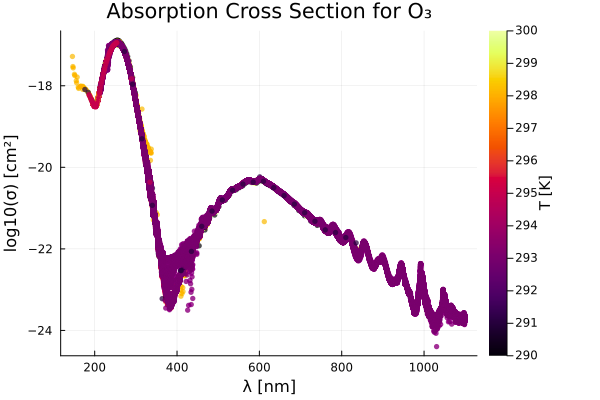
\includegraphics[width=0.85\columnwidth]{heart-chamber/photolysis/O3/cross-section/o3-data.svg}
\end{figure}


\subsection{Quantum Yields}
\subsection{Photolysis Rate Determination}


\section{HEART Chamber Sensing System}



\section{Chemical Data Assimilation}



\section{An Evaluation of Photocatalytic Ionization}



%% \begin{itemize}
%% \item sensor fusion
%% \item photolysis
%% \item docker ingestion framework
%% \item Master Chemical Mechanism
%% \item CRI Mechanism
%% \item AutoChem
%% \item data assimilation
%% \item Overview of all sensor in sensor matrix
%% \item Overview of measurement capabilities (list of species, uncertainty levels, etc...)
%% \item Overview of containerized data acquisition pipeline
%% \item NodeRed
%% \item InfluxDB
%% \item Grafana
%% \item Quarto
%% \item Automatic Alerts
%% \item Automatic Reports
%% \item MCM Implementation in Julia
%% \item Direct computation of Photolysis rates
%% \item Combination with Dr. Lary's AutoChem
%% \item Addition of Ion Chemistry from MIT Lightning disseration
%% \item Visualization of chemical cycles
%% \item SciML methods to infer below detection limits
%% \item Ion Chemistry
%% \item Indoor Air Quality
%% \item Photocatalytic Ionization
%% \end{itemize}





% Begin the bibliography:
\begin{thesisbib}  % <--- THIS LINE IS REQUIRED!
  \bibliography{./references.bib}
\end{thesisbib}  % <-- THIS LINE IS REQUIRED!



\begin{biosketch}
  \textbf{\textcolor{red}{UPDATE REQUIRED!}}
\end{biosketch}


\begin{vita}  % <-- THIS LINE IS REQUIRED!
  \textbf{\textcolor{red}{UPDATE REQUIRED!}}
\end{vita}  % <-- THIS LINE IS REQUIRED!


\end{document}

